% !TEX TS-program = pdflatex
% !TEX encoding = UTF-8 Unicode

% This is a simple template for a LaTeX document using the "article" class.
% See "book", "report", "letter" for other types of document.

\documentclass[11pt]{article} % use larger type; default would be 10pt

%%
%% preamble for knitr output
%%
\usepackage[]{graphicx}\usepackage[]{color}
% maxwidth is the original width if it is less than linewidth
% otherwise use linewidth (to make sure the graphics do not exceed the margin)
\makeatletter
\def\maxwidth{ %
  \ifdim\Gin@nat@width>\linewidth
    \linewidth
  \else
    \Gin@nat@width
  \fi
}
\makeatother

\definecolor{fgcolor}{rgb}{0.345, 0.345, 0.345}
\newcommand{\hlnum}[1]{\textcolor[rgb]{0.686,0.059,0.569}{#1}}%
\newcommand{\hlstr}[1]{\textcolor[rgb]{0.192,0.494,0.8}{#1}}%
\newcommand{\hlcom}[1]{\textcolor[rgb]{0.678,0.584,0.686}{\textit{#1}}}%
\newcommand{\hlopt}[1]{\textcolor[rgb]{0,0,0}{#1}}%
\newcommand{\hlstd}[1]{\textcolor[rgb]{0.345,0.345,0.345}{#1}}%
\newcommand{\hlkwa}[1]{\textcolor[rgb]{0.161,0.373,0.58}{\textbf{#1}}}%
\newcommand{\hlkwb}[1]{\textcolor[rgb]{0.69,0.353,0.396}{#1}}%
\newcommand{\hlkwc}[1]{\textcolor[rgb]{0.333,0.667,0.333}{#1}}%
\newcommand{\hlkwd}[1]{\textcolor[rgb]{0.737,0.353,0.396}{\textbf{#1}}}%
\let\hlipl\hlkwb

\usepackage{framed}
\makeatletter
\newenvironment{kframe}{%
 \def\at@end@of@kframe{}%
 \ifinner\ifhmode%
  \def\at@end@of@kframe{\end{minipage}}%
  \begin{minipage}{\columnwidth}%
 \fi\fi%
 \def\FrameCommand##1{\hskip\@totalleftmargin \hskip-\fboxsep
 \colorbox{shadecolor}{##1}\hskip-\fboxsep
     % There is no \\@totalrightmargin, so:
     \hskip-\linewidth \hskip-\@totalleftmargin \hskip\columnwidth}%
 \MakeFramed {\advance\hsize-\width
   \@totalleftmargin\z@ \linewidth\hsize
   \@setminipage}}%
 {\par\unskip\endMakeFramed%
 \at@end@of@kframe}
\makeatother

\definecolor{shadecolor}{rgb}{.97, .97, .97}
\definecolor{messagecolor}{rgb}{0, 0, 0}
\definecolor{warningcolor}{rgb}{1, 0, 1}
\definecolor{errorcolor}{rgb}{1, 0, 0}
\newenvironment{knitrout}{}{} % an empty environment to be redefined in TeX

\usepackage{alltt}
\newcommand{\SweaveOpts}[1]{}  % do not interfere with LaTeX
\newcommand{\SweaveInput}[1]{} % because they are not real TeX commands
\newcommand{\Sexpr}[1]{}       % will only be parsed by R

%%
%% end of knitr preamlbe
%%


\usepackage[utf8]{inputenc} % set input encoding (not needed with XeLaTeX)
\usepackage{url}

%%% Examples of Article customizations
% These packages are optional, depending whether you want the features they provide.
% See the LaTeX Companion or other references for full information.

%%% PAGE DIMENSIONS
\usepackage{geometry} % to change the page dimensions
\geometry{a4paper} % or letterpaper (US) or a5paper or....
% \geometry{margin=2in} % for example, change the margins to 2 inches all round
% \geometry{landscape} % set up the page for landscape
%   read geometry.pdf for detailed page layout information

\usepackage{graphicx} % support the \includegraphics command and options

% \usepackage[parfill]{parskip} % Activate to begin paragraphs with an empty line rather than an indent

%%% PACKAGES
\usepackage{booktabs} % for much better looking tables
\usepackage{array} % for better arrays (eg matrices) in maths
\usepackage{paralist} % very flexible & customisable lists (eg. enumerate/itemize, etc.)
\usepackage{verbatim} % adds environment for commenting out blocks of text & for better verbatim
\usepackage{subfig} % make it possible to include more than one captioned figure/table in a single float
% These packages are all incorporated in the memoir class to one degree or another...

%%% HEADERS & FOOTERS
\usepackage{fancyhdr} % This should be set AFTER setting up the page geometry
\pagestyle{fancy} % options: empty , plain , fancy
\renewcommand{\headrulewidth}{0pt} % customise the layout...
\lhead{}\chead{}\rhead{}
\lfoot{}\cfoot{\thepage}\rfoot{}

%%% SECTION TITLE APPEARANCE
\usepackage{sectsty}
\allsectionsfont{\sffamily\mdseries\upshape} % (See the fntguide.pdf for font help)
% (This matches ConTeXt defaults)

%%% ToC (table of contents) APPEARANCE
\usepackage[nottoc,notlof,notlot]{tocbibind} % Put the bibliography in the ToC
\usepackage[titles,subfigure]{tocloft} % Alter the style of the Table of Contents
\renewcommand{\cftsecfont}{\rmfamily\mdseries\upshape}
\renewcommand{\cftsecpagefont}{\rmfamily\mdseries\upshape} % No bold!

\usepackage[section]{placeins}
\usepackage{a4wide}
\usepackage{drs}
\usepackage{natbib}
\usepackage{graphicx}
\usepackage{tikz}
\usepackage{tikz-qtree}
\usepackage{linguex}
\usepackage{ulem}
\usepackage{threeparttable}
\usepackage{comment}

%\usepackage[width=.75\textwidth]{caption}

%%% END Article customizations

%%% The "real" document content comes below...

\title{Semantic accesibility and interference in pronoun resolution\\}
\author{TS, JW, JD, RN}


\newcommand{\dependent}[1]{\textit{#1}}
\newcommand{\antecedent}[1]{\textit{#1}}
\newcommand{\distractor}[1]{\textbf{#1}}
\newcommand{\cond}[1]{\textbf{#1}}

\newcommand{\factor}[1]{\textsc{#1}}
\newcommand{\red}[1]{\textcolor{red}{#1}}

%element in memory == item (cf. Jager et al.)




%\date{} % Activate to display a given date or no date (if empty),
         % otherwise the current date is printed 

\begin{document}
\maketitle

\section{Abstract}
[OLD ABSTRACT FROM AMLAP, NEEDS TO BE UPDATED WHEN THE PAPER IS FINISHED]\\

The general view in syntactic literature is that binding constraints can make antecedents syntactically inaccessible. However, several studies showed that antecedents which are ruled out by syntactic binding constraints still influence online processing of anaphora in some stages, suggesting that a cue-based retrieval mechanism has to play a role as well during some stages of anaphora resolution. As in the syntactic literature, in semantic accounts like Discourse Representation Theory (DRT), formal constraints are formulated in terms of accessibility of the antecedent. In DRT, non-referential NPs form inaccessible antecedents, which might thus be expected to be discarded as potential antecedents in an early stage of processing. In an eye-tracking experiment we generalized these findings by looking at the role of accessiblilty in pronoun resolution in online sentence processing of inter-sentential anaphoric relations. The results suggest that accessibility has an effect on pronoun resolution from early on: inaccessible antecedents were ruled out as a possible resolution in an early stage, which would be predicted by theories like DRT. This suggest that, unlike the general view of DRT as a purely semantic theory, it can also be used in a more cognitive setting.\\


\section{Introduction}
Sentence comprehension and production undoubtedly relies on working memory and nowhere is this reliance more visible than in case of comprehension of so-called \emph{dependents}: elements whose interpretation and/or form depends on another linguistic item. An example of a dependent is the verb \textit{talks} in \Next, whose form depends on the subject \textit{John}. The verb also depends on the subject for its interpretation, in particular, the subject specifies how one of the roles of the verb, the agent, should be understood. Thus, to arrive at the correct form and interpretation of the verb, a memory retrieval has to take place and the fitting item has to be recalled.

\ex. John always talks about Mary.

One prominent line of research argues that the recall of the correct item is a cue-based retrieval mechanism: it accesses the items in memory that match the dependent in retrieval cues \citep{mcelree00, dyke+03, mcelree+03, lewis+06, dyke07, vasishth+08, wagers+09, dillon+13, jager+17, nicenboim+18}. In the case above, \Last, there are three features that could arguably guide the retrieval. In particular, the item has to be \emph{3rd person}, \emph{singular} and \emph{subject}. All of these features are present on the proper noun \textit{John} and therefore, they can be used to access it.

While cue-based retrieval became well accepted and maybe even the default model in case of agreement resolution, as in \Last, and for other intra-clausal dependencies, it is far from clear that it should be used to model all dependent-triggered retrievals. In particular, very little is known about dependents that operate across a discourse. This is the topic of the current paper. We will investigate memory retrieval needed for pronoun resolution in short (up to three sentence-long) discourses. In the next section, we will summarize the main facts about cue-based retrieval. After that, we will discuss the research that studied dependencies of pronoun from the perspective of cue-based retrieval and is thus directly relevant to ours.

%%%%%%%%%%%%%%%%%%%%%%%%%%%%%%%
\section{Main facts about cue-based retrieval}
\label{sec_cuebased}
%%%%%%%%%%%%%%%%%%%%%%%%%%%%%%%

Cue-based retrieval in dependencies has currently been implemented in two models (cf. \citealt{nicenboim+18}): the direct-access model, see \cite{mcelree00}, and activation-based model, see \cite{lewis+05}. Disregarding the implementation details of the models, we will focus on three assumptions that have driven the research in the study of dependency and memory:

\begin{enumerate}
    \item \emph{Cue-based retrieval is error prone}: when encountering the dependent, what might be recalled is a distractor, which is an item in memory that does not fully match the cues triggering the retrieval.
    \item \emph{Error in recall is cue-dependent}: The chance that the distractor is erroneously recalled increases with the number of features in which the distractor does match the right cues.
    \item \emph{Retrieval time is sensitive to memory fan of cues}: The time to retrieve an item using some cue $X$ increases with the number of items in memory that also have $X$ (this assumption is present in activation-based models, but absent in direct-access models)
\end{enumerate}
            
\noindent We will show how these assumptions work on the paradigm in \Next.

\ex.
\a. The key to the cabinets always is \ldots
\b. The key to the cabinet always is \ldots
\c. The key to the cabinet always are \ldots
\d. The key to the cabinets always are \ldots

In \Last, the verb-subject dependency requires that the subject, the phrase \textit{the key to the cabinet(s)} be recalled. Following common terminology, we call this phrase a target. The other noun phrase present in the clause, \textit{the cabinet(s)}, is the distractor. In \Last[a], the target fully matches and the distractor matches only in its \emph{3rd person} feature. The match of the distractor is increased in \Last[b]: in this case, the distractor matches the verb in person and number. Thus, it is expected that the distractor is more likely erroneously recalled here (assumption 1 \& 2). If, at least in some of these instances, people introspect this recall and attempt to correct it, the slowdown due to repair is predicted in \Last[b] compared to \Last[a]. Furthermore, an independent source of slowdown is predicted in activation-based models because the feature \emph{sg number} is shared between the subject and the distractor, see assumption 3. In \Last[c] and \Last[d], the subject mismatches the number feature and consequently, the sentence is ungrammatical. If, at least in some of these instances, people do not introspect this recall and do not correct it, it is predicted that \Last[d] should be faster than \Last[c]. This is because in \Last[d], the distractor partially matches with the dependent and thus it is more likely to be erroneously recalled and treated as the correct antecedent (due to assumptions 1 \& 2) compared to \Last[c]. The recalling will also be faster because in \Last[d], the number feature \textit{pl} is present only once and thus, the fan is smaller for that cue than in \Last[c] (assumption 3 for activation-based models).

The predictions of the models have been partially confirmed. It has repeatedly been found that ungrammatical cases in which the verb is in plural are read faster when the distractor matches in number, i.e., \Last[d] leads to faster reading times than \Last[c] (cf. \citealt{jager+17} for literature review and Bayesian meta-analysis). While the slowdown in \Last[b] compared to \Last[a] has not been observed for this particular construction, the effect has been found in other examples of verb-subject dependencies (cf. \citealt{jager+17}).

One limit that cue-based retrieval models have is that it is hard to extend them to cases in which relational information plays a role in establishing a dependency. Consider \Next. One dependency in this example is between the reflexive \textit{himself}, which is dependent in its form and interpretation on the subject \textit{John}.

\ex. John should tell Bill about himself.\label{ex2_refl}

Two constraints are at work in establishing the antecedent of the reflexive: the antecendent has to carry the feature \emph{masculine} and it must be \emph{more prominent} than the reflexive and part of the same clause as the reflexive (Principle A, see \cite{chomsky81, reinhart+93}). Let us focus on the second, relational information, which can also be stated as requiring that the antecedent is higher on the prominency hierarchy of intra-clausal arguments than the dependent. The hierarchy can be expressed as a hierarchy of arguments within one clause, or somewhat more abstractly, as a c(onstituent)-command relation in a syntactic tree\footnote{A phrase X c-commands a phrase Y if and only if Y is contained within X's sister} (cf. \citealt{reinhart83}, and \citealt{buring05} for discussion) contained within one clause. We will use the c-command relation here. Translating \Last into the tree structure, see Fig.~\ref{fig_tree1}, we can see that the subject \textit{John} c-commands the object \textit{Bill} and the reflexive. The object also c-commands the reflexive. Thus, it is predicted that the reflexive can have either \textit{John} or \textit{Bill} as its antecedent.

\begin{figure}
    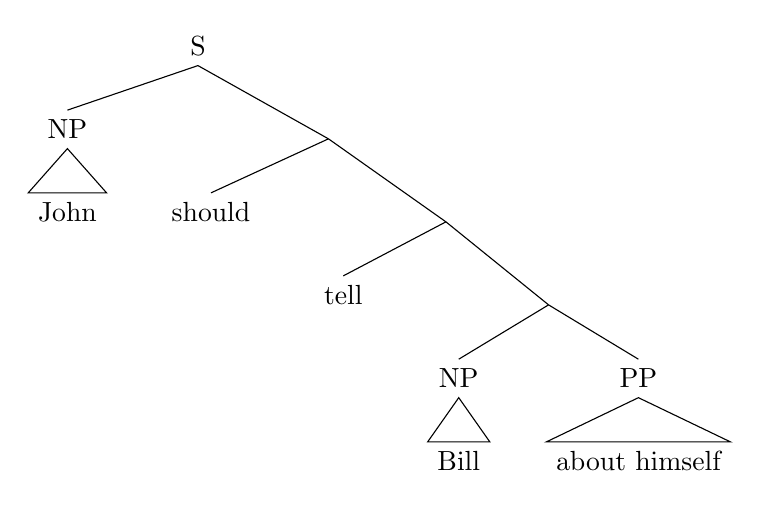
\begin{tikzpicture}[level distance=30pt, sibling distance=20pt]
        \Tree[.S [.NP \edge[roof]; {John} ] [ [.should ] [ [.tell ]  [ [.NP \edge[roof]; {Bill} ] [.PP \edge[roof]; {about himself} ] ] ] ] ]
    \end{tikzpicture}
    \caption{Hierarchy for the sentence \ref{ex2_refl}\label{fig_tree1}}
\end{figure}

The problem is that c-command (or prominency) is a relational notion and thus, it cannot be inherent to any element, unlike features like gender or number. To see that, note that while information such as gender or number on an element exists irrespective of what the dependent is, whether some element c-commands the dependent relies on the position of the dependent. For example, direct objects c-command dependents when dependents are adjunct PPs, but they are c-commanded by dependents when these are subjects. In a right-branching structure as the sentence in Fig.~\ref{fig_tree1} above, the first word (\emph{John} in this case) c-commands all other terminal nodes in the tree, but this will not be known until after all these terminal nodes are encountered. To fully specify the c-command relation as a feature, we would have to assume that the value of the c-command feature of \emph{John} gets updated every time a new word is read. This would put unrealistic demands on the parser as it would entail that each time a new word is read, a retrieval has to be launched to update the c-command feature of all preceding items. This therefore poses a challenge for cue-based retrieval. To put it differently, cue-based retrieval requires that the dependent triggers retrieval based on cues. However, whether some element c-commands the dependent or not is not known until the dependent itself is encountered and therefore, it is hard to see how any element could be endowed with this information in the memory before the actual retrieval takes place.

On the empirical side, it has been argued that reflexives do not show the pattern predicted by cue-based retrieval. For example, \cite{dillon+13} compared the reading profile of agreement dependencies, \Next[a], and reflexive dependencies, \Next[b].

\ex. \a. The new executive who oversaw the middle manager(s) apparently was/*were dishonest about the company's profits.
\b. The new executive who oversaw the middle manager(s) apparently doubted himself/
*themselves on most major decisions.

In two eye-tracking studies, they found a contrast between \Last[a] and \Last[b]. First, it was confirmed that the plural distractor, \textit{the middle managers}, decreased reading times of the predicate with the incorrect agreement (\textit{were dishonest}) compared to the singular distractor. This is in line with cue-based retrieval and follows from the three assumptions as discussed above. Interestingly, the same pattern was not observed for \Last[b]: the plural distractor did not affect reading times of the predicate with the incorrect reflexive (\textit{doubted themselves}). This finding is further supported by the Bayesian meta-analysis reported in \cite{jager+17}, which showed that inaccessible distractors do not interfere with the resolution of reflexive dependencies.

The role of prominency in retrieval also plays a role in case of pronoun resolution. In particular, it is known that quantificational distributive expressions like \textit{no + noun phrase(NP)}, \textit{every + NP}, \textit{each + NP}, can only antecede pronouns that they c-command \citep{heim82, reinhart83}. In contrast to that, referential expressions like \textit{the + NP}, \textit{a + NP} can antecede pronouns that they do not c-command. The contrast is shown in \Next, from \citep{heim82}. \Next[a] is grammatical under the interpretation that \textit{he} refers back to \textit{the soldier} because no c-command is required to establish this relation. \Next[b] is ungrammatical under the interpretation that \textit{he} has \textit{no soldier} as its antecedent because the latter does not c-command the former (c-command does not span across clause boundaries).

\ex. \a. The soldier has a gun. Will he attack?
\b. No soldier has a gun. *Will he attack?


This contrast has been used in the study of \cite{kush+15}. What they compared was a case in which the referential antecedent either matched or mismatched the pronoun in gender (\Next[a]-\Next[b]) with a case in which the quantificational antecedent matched or mismatched (\Next[c]-\Next[d]).

\ex.
    \a. \cond{Referential, Match}\\
    The troop leaders that \antecedent{the girl scout} had no respect for had scolded \dependent{her} after the incident at scout camp.
    \b. \cond{Referential, Mismatch}\\
    The troop leaders that \antecedent{the boy scout} had no respect for had scolded \dependent{her} after the incident at scout camp.
    \b. \cond{Quantificational, Match}\\
    The troop leaders that \distractor{no girl scout} had respect for had scolded \dependent{her} after the incident at scout camp.
    \b. \cond{Quantificational, Mismatch}\\
    The troop leaders that \distractor{no boy scout} had respect for had scolded \dependent{her} after the incident at scout camp.


They observed that in early and late measures referential mismatch slowed down reading compared to referential match. Since in case of referential mismatch, there was no antecedent present for the pronoun, the slowdown can straightforwardly be explained as showing that readers did not know how to resolve the pronoun in \Last[b] compared to \Last[a]. Interestingly, in early measures, the effect was reversed for quantificational antecedents, i.e., matching quantificational antecedents caused a slowdown in the reading of the pronoun and the subsequent text compared to mismatching quantificational antecedents. This is unexpected from the perspective of cue-based retrieval and the assumptions listed above. If anything, we would expect the opposite effect: quantificational match should cause a speed-up compared to quantificational mismatch. This is for the same reason that non-subjects could speed up the processing of verb agreement when they partially matched the agreement in morphological cues, see \LLast[a]. Thus, we see that cue-based retrieval is not supported in this case.

One challenge for this study is that it is not clear to what extent it is correct that quantificational noun phrases can only antecede pronouns that they c-command. In an off-line acceptability task carried out in \cite{kush+15} the referential mismatch was judged as significantly worse than the referential match. This can be explained from the fact that in the mismatch case, \Last[b], no referent is available for the pronoun. However, the quantificational mismatch was also judged as worse than the quantificational match (the effect was marginally significant). The fact that participants penalized sentences in which the quantificational noun phrase mismatched the pronoun strongly suggests that they did consider it as a possible antecedent for the pronoun. In another off-line study in which participants were asked about their interpretation of the pronoun, in 28\% of responses participants indicated that they resolved the pronoun as having the non-c-commanding quantificational noun phrase as the antecedent. Both off-line studies thus cast serious doubts on the assumption that quantificational noun phrases that do not c-command pronouns cannot provide antecedents for them.

Secondly, the research line of \cite{kush+15} cannot be extended to pronoun resolution in discourse. The reason for this is that c-command is a strictly intra-sentential relation and thus, it cannot be used to study pronoun resolution across sentences. For the purpose of pronoun resolution in discourse, we will therefore need a different approach. This is introduced in the next section. Afterwards, we will see that the proposed approach allows us to avoid the problem of \cite{kush+15} discussed above: we will be able to develop a design in which quantificational noun phrases in specific relational constellations cannot serve as antecedents for pronouns, not even marginally so. Because our approach provides cases in which the antecedenthood of noun phrases is clear, this provides a more suitable starting point for the study of recall in the comprehension of pronouns.

\section{Discourse and pronouns}

When hearers comprehend a sentence, they rarely interpret it in vacuum. Rather, they understand it in its context. In theories of meaning called dynamic semantics, pieces of text, e.g., sentences, are seen as instructions to update context and the main focus is to understand what properties such an update has. The dynamic semantic framework that is arguably most popular and accessible, Discourse Representation Theory (cf. \citealt{kamp81, kamp+93}), assumes that a hearer builds a mental model during comprehension. The mental model, called a discourse representation structure, is a representation that consists of two pieces of information: (i) discourse referents, which are arbitrary labels, pegs that serve as pointers to entities under discussion in that discourse, (ii) discourse conditions, i.e., what information the discourse provides on those entities. For example, assuming that \Next is the starting point of discourse, hearer's comprehending would lead to the construction of a mental model representation in \NNext. This representation shows in the top part the information that two entities were introduced in this short discourse, labelled (arbitrarily) as $x$ and $y$. Furthermore, three pieces of information are collected on those entities, written as conditions on $x$ and $y$ in the bottom part.

\ex. A man read a book.

\ex. \drs{x y}{$x$ is a man\\$y$ is a book\\$x$ read $y$}

When this sentence is followed by another one, e.g., \Next, \Next is nothing more than instructions to update the current representation. Pronouns, in turn, are interpreted just as old discourse referents, i.e., pegs that must have been introduced previously (e.g., $x$ and $y$ in this example). The resulting discourse representation structure is in \NNext. The contribution of the second sentence is in the last line of the discourse representation structure in \NNext.

\ex. He liked it.

\ex. \drs{x y}{$x$ is a man\\$y$ is a book\\$x$ read $y$\\$x$ liked $y$}

Discourse Representation Theory allows for embedding one discourse representation structure inside another. Intuitively, this can be understood as a situation in which inside one discourse, another (sub-)discourse is being developed. Discourse Representation Theory precisely specifies under which conditions sub-discourses can be introduced \citep{kamp+93}. These conditions are not particularly relevant for us, it suffices to note that negation and negative quantifiers are one trigger of sub-discourses.

An example is given in \Next, which would be represented as in \NNext. The sub-discourse is preceded by \textbf{not}, signalling that the sub-discourse must not be true.

\ex. A man read no book.

\ex. \drs{x}{$x$ is a man\\\textbf{not} \drs{y}{$y$ is a book\\$x$ read $y$}}

Importantly, discourse referents introduced in sub-discourses are not accessible outside of these sub-discourses. This condition restricts potential antecedents for pronouns. More concretely, it has a straightforward effect for \LLast. Since a new sentence updated the largest discourse representation structure, pronouns appearing in a new sentence could not be interpreted as $y$, i.e., as a book. The only other discourse referent is $x$, so the only possible interpretation for pronouns is $x$, which could be paraphrased, given the conditions in \Last, as `the man who read no book'. In particular, suppose that \LLast is followed by \Next. This would lead to the update in \NNext. Here, the object of \textit{liked} cannot be assigned a representation since the only available discourse referent is $x$ and $x$ is a man, so it cannot be referred back to by \textit{it}. Thus, it is predicted by Discourse Representation Theory that the pronoun in this follow-up discourse will receive no interpretation. This prediction has been argued to match people's intuitions (cf. \citealt{kamp+93}).

\ex. He liked it.

\ex.  \drs{x}{$x$ is a man\\\textbf{not} \drs{y}{$y$ is a book\\$x$ read $y$}\\$x$ liked ??}


In sum, Discourse Representation Theory is a semantic framework that provides (i) the interpretation of discourses and (ii) general conditions specifying whether a particular discourse is well-formed. With respect to the latter, Discourse Representation Theory argues that pronouns can only be resolved to those discourse referents that are accessible. Like c-command, accessibility in Discourse Representation Theory is a relational notion. However, unlike c-command, accessibility spans over sentences across the complete discourse. We can thus use accessibility to study how a condition on discourse well-formedness affects pronoun resolution in processing. Furthermore, as we will see, using insights from Discourse Representation Theory gives us a handle on the problem that plagued \cite{kush+15}, that is, we will be able to construct discourses in which pronoun resolution to inaccessible antecedents is clearly impossible.

We will now study pronoun resolution in discourse and the role of accessibility in establishing of the right antecedent for pronouns in three experiments.


\begin{comment}
\begin{itemize}
\item Problem with Kush et al. (2015): their `inaccessible' condition is not really inaccessible.
\item Our experiment is new because it goes beyond sentence borders. 
\end{itemize}
\end{comment}


\section{Experiments}

Three experiments were conducted with the materials we developed for this study. Therefore, we will first describe the materials, before going into detail about the separate experiments.

\subsection{Materials}

The materials for the experiments are in Dutch. All target items have the same structure, consisting of short storylines of 2 sentences. In the first sentence of each item, two discourse referents are introduced: the first one is introduced by a noun phrase that appears in the subject position. The second one is introduced by a noun phrase in the object or prepositional object position. The second sentence contains an anaphoric pronoun. The interpretation of this pronoun is therefore dependent on the discourse referents in the first sentence. Given Discourse Representation Theory, discussed above, whether a discourse referent can be used to resolve a pronoun depends on whether the discourse referent is accessible to the pronoun or not. In our setup, the subject was a definite noun phrase and its discourse referent was always accessible. The second discourse referent, the object, was either introduced by an indefinite (in that case, it was accessible) or it was introduced by a negative quantifier (in that case, it was inaccessible). Like Kush et al. (2015), we made use of gender features to look into the effect of the accessible and inaccessible antecedent on the resolution of the pronoun. That is, we manipulated the gender of the subject and the object, thereby creating conditions in which their gender either matches or mismatches the gender features of the pronoun. 

The subject had to be a character which clearly targets one gender, to make it possible to create a mismatch with the pronoun. However, it had to be possible to reinterpret the character as the other gender as well, because otherwise there is no resolution for the pronoun in case of a mismatching and/or inaccessible object. In that case, no anaphoric relationship can be established in a substantial amount of the experimental items, which might lead participants to give up on establishing an anaphoric relation between the pronoun, or employ other alternative parsing strategies. The same strategy has been employed in Sturt (2003). The choice of the male-biased nouns was partly based on the nouns used by Sturt (2003) and mostly dependent on the fact that in Dutch, gender-biased nouns which can also be interpreted as the other gender are always male-biased. There are basically no nouns which are stereotypically interpreted as female but can also refer to a male. To make sure that the nouns we selected are male-stereotypical, but when necessary they must be used to refer to females since there is no other specific word form, we only included nouns that did not have a female-gender marked equivalent in Dutch (such as \textit{loodgieter} `plumber'), or for which a female version was used in less than 0.7\% of the time in the `Corpus Hedendaags Nederlands' (http://corpushedendaagsnederlands.inl.nl). 

The second antecedent, the grammatical object of the first sentence, could refer to a non-ambiguous male or female character (e.g., brother/sister and other kinship terms). The anaphoric pronoun in the second sentence was either male or female. This pronoun could either match or mismatch the subject's gender (SUBJECT MATCH vs. SUBJECT MIS) and the object's gender (OBJECT MATCH vs. OBJECT MIS). Furthermore, the object was preceded either by \textit{een} ‘a’ (a REFERENTIAL or accessible antecedent) or by the negative quantifier \textit{geen} ‘no’ (a NON-REFERENTIAL or inaccessible antecedent). This creates a total of $2*2*2$ conditions. An overview of all conditions illustrated with an example stimulus is given in Table \ref{tab:conditions}.


\begin{table}\small
\center
\caption{\label{tab:conditions}\footnotesize{Overview of the experimental conditions with an example}}\vspace{-3mm}
\hspace*{-1cm}\begin{tabular}[width=0.5\textwidth]{l|p{0.6\linewidth}}
\hline
 Condition & Example stimulus \\\hline\hline 
ACC*subjMATCH*objMATCH & De professor heeft een zoon. De laatste paar jaar werkte hij helaas op alle feestdagen.  \\
ACC*subjMATCH*objMIS & De professor heeft een dochter. De laatste paar jaar werkte hij helaas op alle feestdagen.  \\
ACC*subjMIS*objMATCH & De professor heeft een dochter. De laatste paar jaar werkte zij helaas op alle feestdagen.  \\
ACC*subjMIS*objMIS & De professor heeft een zoon. De laatste paar jaar werkte zij helaas op alle feestdagen.  \\
INACC*subjMATCH*objMATCH & De professor heeft geen zoon. De laatste paar jaar werkte hij helaas op alle feestdagen.  \\
INACC*subjMATCH*objMIS & De professor heeft geen dochter. De laatste paar jaar werkte hij helaas op alle feestdagen.  \\
INACC*subjMIS*objMATCH & De professor heeft geen dochter. De laatste paar jaar werkte zij helaas op alle feestdagen.  \\
INACC*subjMIS*objMIS & De professor heeft geen zoon. De laatste paar jaar werkte zij helaas op alle feestdagen.  \\
\hline
\multicolumn{2}{p{0.99\linewidth}}{‘The professor has [a/no] [son/daughter]. The past few years, [he/she] unfortunately had to work during all the holidays.’}\\
\end{tabular}
\end{table}





\subsection{Experiment 1a: Resolution task}
\subsubsection{Participants}
28 participants participated in an online study.

\subsubsection{Design \& Procedure}
To test whether the use of a negative quantifier indeed blocked the accommodation of the object NP as an antecedent for the pronoun, we carried out an online comprehension study. The items were presented one by one, along with a comprehension question which targeted the interpretation of the pronoun. Participants could choose between three options: the subject, the object, or `other'. 


\subsubsection{Results \& Discussion}

\begin{threeparttable}
\caption{\label{tab:resolutiontask}Results of the resolution task}
       	\begin{tabular}{ll | lll}

	\multicolumn{2}{c}{Condition} & \multicolumn{3}{c}{Response} \\
	Subject & Object & Subject & Object & Other \\
	\hline
	Match & Match & .94 & .03 & .03 \\
	Match & Mismatch & .96 & 0 & .04 \\
	Mismatch & Match & .88 & .07 & .05 \\
	Mismatch & Mismatch & .97 & 0 & .03 \\\\
	\end{tabular}
\end{threeparttable}
\bigskip

The results, summarized in Table \ref{tab:resolutiontask}, show that participants almost always chose the subject as resolution for the pronoun, and almost never chose the object. This means that the negative quantifier indeed blocked the accommodation of the object NP as an antecedent for the pronoun. Based on this, we can assume that the object is really inaccessible. No significant effect of target and distractor gender on selection of the subject was found. 



\subsection{Experiment 1b: Acceptability Judgement Task}
\subsubsection{Participants}
Sixty-eight participants (36 female) participated in the online experiment. All of them were aqcuired from the online questionnaire platform Prolific. Their mean age was 27.21 years (SD: 8.07; range: 18-53). All participants reported to be native speakers of Dutch; none of them reported to suffer from dyslexia or other reading problems. The task lasted for 10-15 minutes and participants were rewarded with 3 euros.

\subsubsection{Design \& Procedure}
We carried out an online acceptability judgement task to test the acceptability of the stimuli in all conditions. The items were presented one by one, together with a 7-points Likert scale on which participants could indicate how much sense the context made to them (1 = completely ununderstandable, 7 = perfectly understandable). Items were divided over 8 lists via a Latin square and were randomly presented, interspersed with 48 fillers. Half of these fillers were contexts we expected to receive high scores, the other half we expected to receive low scores. Besides leading the attention away from the goal of the experiment, the fillers served to check whether participants were paying enough attention. The mean score of each filler was calculated and all scores that deviated 3 or more points from the mean were marked as an error. The mean number of errors over all participants was 2.63. After visual inspection of the data, we decided to exclude participants with 6 or more errors, which led to the exclusion of 12 participants in total.

\subsubsection{Results \& Discussion}
Table \ref{tab:descriptives} shows the descriptives per condition. Results were analyzed with Cumulative Link Mixed Models in R. Sum contrast coding was applied to the different conditions, associating a positive quantifier (een) with -1 and a negative quantifier (geen) with 1; for both Subject and Object the Mismatch condition was coded with -1 and the Match condition with 1. Results of the analysis of the full dataset are summarized in Table \ref{tab:fullmodel}. 



\begin{threeparttable}
\caption{\label{tab:descriptives}Mean and standard deviation of the scores per condition}
\begin{tabular}{lll|ll}
	\multicolumn{3}{c}{Condition} & \multicolumn{2}{c}{Response} \\
	Quantifier & Subject & Object & Mean & SD \\
	\hline
	Een & Match & Match & 4.374 & 1.832\\
	Een & Match & Mis & 4.074 & 1.822  \\
	Een & Mis & Match & 4.853 & 1.779  \\
	Een & Mis & Mis & 3.638 & 1.765 \\
	Geen & Match & Match & 3.522 & 1.894  \\
	Geen & Match & Mis &  3.568 & 1.859  \\
	Geen & Mis & Match &  3.026 & 1.727  \\
	Geen & Mis & Mis & 3.312 & 1.899   \\\\
	\end{tabular}
\end{threeparttable}



\begin{threeparttable}
\caption{\label{tab:fullmodel}Overview of the results of the full dataset}
\begin{tabular}{lllll}
	Condition & Estimate & Std. Error & z value & Pr($>|z|$) \\
	\hline
Quan       &             -0.308   & 0.075 & -4.128& 3.66e-05 ***\\
Subj        &            0.064  &  0.039 & 1.665 & 0.096 .  \\
Obj         &            0.114  &  0.038 & 2.999&  0.003 ** \\
Quan*Subj &          0.079  &  0.024 & 3.208 & 0.001 ** \\
Quan*Obj  &          -0.165  &  0.025  & -6.691 &2.21e-11 ***\\
Subj*Obj   &        -0.044  &  0.025 & -1.788  &0.074 .  \\
Quan*Subj*Obj &  0.108  &  0.025 &  4.375& 1.22e-05 ***\\\\
\end{tabular}
\end{threeparttable}


The main effect of Quantifier shows that items with a negative quantifier scored significantly lower than items with a positive quantifier. A main effect of Object was found as well: items with a mismatching object received a lower score than items with a matching object. For Subject, the effect was in the same direction but did not reach significance. In the interactions we see that the effects of both Subject and Object depend on the type of quantifier. It appears that a mismatching subject only had a negative effect in combination with a negative quantifier. For Object, this was the other way around: a mismatching object only had a negative effect in combination with a positive quantifier. This contrast is even more clearly visible after splitting the data into subsets by quantifier, as in Table \ref{tab:byquan}. 


\begin{threeparttable}
\caption{\label{tab:byquan}Overview of the results split by quantifier}
\begin{tabular}{llllll}
Quantifier	& Condition & Estimate & Std. Error & z value & Pr($>|z|$) \\
	\hline
Geen &Subj  &       0.236   & 0.059 & 3.962& 7.44e-05 ***\\
 &Obj    &        -0.081 &   0.059 &  -1.373 & 0.170 \\
 &Subj*Obj & 0.122   & 0.060  & 2.031  &0.042 *\\
\hline
Een&Subj &          -0.019    &0.085  & -0.226 &   0.821    \\
&Obj    &       0.493   & 0.100  &4.926 &8.38e-07 ***\\
&Subj*Obj& -0.274  &  0.061 &  -4.516 &6.32e-06 ***\\\\
\end{tabular}
\end{threeparttable}

When the item contained a negative quantifier and the subject mismatched the pronoun, the item scored significantly lower, compared to when the subject matched. The object, which was inaccessible in this setting, did not have such an effect. The interaction of Subject and Object, however, shows that the effect of Object differed for matching and mismatching subjects. As can be seen in Table \ref{tab:descriptives}, there is no clear difference between matching and mismatching objects when the subject matched, but when the subject mismatched, a mismatching object involved a \textit{higher} score than a matching object. 


%subj match: $\beta = 0.050(0.085), t = 0.556$
%subj mis: $\beta = -0.205(0.087), t = 0.018$


When the item contained a positive quantifier, there was no main effect of Subject. However, there was a main effect of Object: a mismatching object led to a significantly lower score, compared to a matching object. As illustrated by Table \ref{tab:descriptives} the interaction effect of Subject and Object additionally shows that the negative effect of a mismatching object was much larger when the subject mismatched as well, compared to when the subject matched. 


%subj match $\beta = -0.194(0.084), t = 0.021$ 
%subj mis $\beta = -0.79(0.145), t = 3.61e-08$


We expected that in all conditions in which there was a straightforward resolution for the pronoun, the context would receive a relatively high acceptability score, while we expected lower scores for contexts in which there was no straightforward resolution (note that in the end, the subject could always resolve the pronoun but in the case of a mismatching gender this required additional reasoning). This means that in situations where the subject matched, (straightforward) resolution was always possible. The same holds for situations where the object matched and was accessible. Together, this would mean that we expect the lowest scores in conditions with mismatching subject and mismatching object, or mismatching subject and inaccessible object. In case the object was inaccessible, we expected that an effect of gender mismatch would be smaller or absent. 

The results largely reflect these expectations. In situations where the object was accessible, a gender mismatch involved lower scores, especially when the subject mismatched the pronoun's gender as well (as this means there was no straightforward resolution for the pronoun). In the cases where the object was inaccessible, however, a gender mismatch did not lead to a lower score. When the subject mismatched, the score was even higher for a mismatching inaccessible object, compared to a matching object. A possible explanation for this could be that matching properties of an inaccessible element have a negative effect on acceptability, while they have a positive effect when the element is accessible. This is supported by the most notable difference in mean scores summarized in Table \ref{tab:descriptives}. Although no hard conclusions can be drawn from these raw scores, they show that the accessible SubjMis-ObjMatch condition received the highest mean score (4.853), while the inaccessible SubjMis-ObjMatch condition received the lowest mean score (3.026). In both cases, the object is the only element that matches the pronoun's gender, but apparently, this only improves acceptability when it is accessible. An additional possible explanation is that this difference has to do with the markedness of the nouns. In the SubjMis-ObjMatch condition, the object is always female. This female noun, which is more specific than the male alternative and hence more marked, could effect the score in a negative way when it is combined with a negative quantifier. 


\newpage

\subsection{Experiment 2: Eye-tracking Experiment}



\subsubsection{Participants}
Forty-eight participants (41 female) participated in the experiment. Most of them were bachelor's or master's students at Utrecht University; all of them were acquired from the UiL OTS participants database. The mean age was 23.37 years (SD: 3.01; range: 19-33). All participants were native speakers of Dutch. None of them reported to suffer from dyslexia, severe eye abnormalities, or other reading problems. Participants with glasses or contact lenses were allowed to participate if their vision was corrected-to-normal. Participants were rewarded with 10 euros. 



\subsubsection{Materials and design}
The experiment contained 32 target items and 48 fillers. The mean length of the target items was 102.4 characters; the mean length of the fillers was 109.1 characters. The target items all had the same structure, consisting of nine Interest Areas (IAs). This structure is illustrated in Table \ref{tab:targetitem}. 


\begin{table}[ht]\small
\center

\caption{\label{tab:targetitem}\footnotesize{Example of the structure of a target item}}\vspace{-3mm}
\hspace*{-1cm}\begin{tabular}[width=0.5\textwidth]{llp{2.1cm}p{3cm}p{3cm}p{1.5cm}l}
\hline
IA1 & IA2 & IA3 & IA4 & IA5 & IA6 & IA7 \\
\hline
subject & verb & object & introductory part & verb + pronoun & 3 following words & wrap-up\vspace{4mm}\\
\textit{De professor} & \textit{heeft} & \textit{[een/geen] [zoon/dochter].} & \textit{De laatste paar jaar} & \textit{werkte [hij/zij]} & \textit{helaas op alle} & \textit{feestdagen}\\\\
\multicolumn{7}{l}{‘The professor has [a/no] [son/daughter]. The past few years, [he/she] unfortunately had to work during}\\
\multicolumn{7}{l}{all the holidays.’}\\
\hline
\end{tabular}\hspace*{-1cm}
\end{table}

The fillers were short storylines too, consisting of 2 or 3 sentences. Some fillers only contained a subject; some contained a subject and an object. In the second and/or third sentence a reference to one of the characters was made, either by a pronoun or by a proper name/noun.  Target items were divided over 8 lists via a Latin square and together with the fillers presented in a unique random order for each participant. Maximally 2 items of the same condition could follow each other. Half of the fillers and half of the target items were followed by comprehension questions, which could be answered by yes or no. Each list started with a practice block. The practice block had a fixed order and consisted of four practice items, two of which were followed by a comprehension question (one to be answered with yes; one with no). 

\subsubsection{Procedure}

The participants performed an eye-tracking task in the UiL-OTS lab at Utrecht University. The experiment was programmed in ZEP (version 1.16) and the eye-tracking system used was Eyelink 1000, combined with a target sticker on participants' forehead and a Beexy button box. Participants were seated in front of a PC monitor in a sound-proof, dimly lit booth. The distance to the screen was approximately 60 centimeters. After they read the study information and signed the consent form, the chair and camera were adjusted to the appropriate heighth/angle. Because of the COVID-situation at that time, this all had to be done with taking the social distance into account, which meant that it took more time than usually and that participants were sometimes asked to leave the booth to allow the experiment leader to go inside and make adjustments to the equipment. 

Once the participants were seated in an appropriate position and read the instruction screen of the experiment, the first calibration and validation were performed, followed by the practice block. After a final opportunity to ask questions, a new calibration and validation were performed and the main experiment was started. In total, the experiment took 30-45 minutes, dependent on how long it took to obtain a good calibration.

The stimuli were horizontally aligned to the left side of the screen and consisted of multiple lines. Each line could maximally contain 70 characters. It was ensured that the critical region (the region with the pronoun) was always preceded by and followed by several words on the same line, making it appear roughly in the middle of the line. Before each stimulus was presented, a fixation trigger containing a drift correction was presented at the coordinates of the beginning of the stimuli. In this way it was ensured that participants fixated on the position of the beginning of a stimulus before it was presented, and a new calibration could be performed if necessary. 

Participants were instructed to press the lower (middle) button on the button box to proceed to the next stimulus. When a stimulus was followed by a comprehension question, they could answer it with `no' by pressing the left button, and with `yes' by pressing the right button. This information was visible at the bottom of the screen for all questions, to avoid confusion. 


\subsubsection{Data analysis}
One participant was excluded from the analysis due to poor calibration; no participants were excluded based on the comprehension questions (all participants scored above 85\% correct). The results were manually corrected for drift with the program Fixation by a student assistant, who did not know the purpose of the experiment and did not understand Dutch. In this way it was ensured that this process remained independent of any expectations based on the theory. Two items were generally excluded from the analysis due to typos that were discovered afterwards. In 6 participants, 1 or 2 items were excluded due to poor calibration or the absence of fixations (11 items in total).

All 7 regions of interest were analyzed. The dependent variables were First Fixation Duration, First Pass, Right-Bounded, Regression Path and Regressions (Early measures) and Re-readings, Re-reading Duration, and Total Times (Late measures). The independent variables were Subj (MATCH/MIS), Obj (MATCH/MIS), and Quan (EEN/GEEN). Data points without fixations were excluded from the analyses. \\

The data are analyzed in the Bayesian paradigm using hierarchical models
\citep{gelman2003bda,gelman2006data,mcelreath2018statistical,nicenboim2021introd_bayes_data}.
Before turning to the actual experiments, we will here briefly summarize
general properties of the models to be considered.

In Bayesian data analysis one specifies the likelihood, and the prior
distributions over parameters of interest. The analysis results in
posterior probability distributions of plausible values for a given
model and data. We report medians and 95\% credible intervals (CRI),
i.e.~the range of values for which we can be 95\% certain that the true
effect lays therein. An important feature of Bayesian analysis is
uncertainty highlighting, and the width of the intervals can be used to
assess uncertainty of the parameters' values.

Beside two special cases the prior distributions used for modelling were
``weakly informative'' \citep{gelman2003bda} p.~55. This means they
contain little real-world knowledge and a priori they do not exclude any
observable values. With the exception of the two already mentioned
cases, the prior distributions were also constructed in such a way which
would not pull the results in any direction. We wanted to remain
agnostic both about the size and the direction of the effects. The
details of the prior distributions are specified when discussing each
experiment.

Unless explicitly stated otherwise, models used 4 sampling chains with
4000 samples drawn from each chain. Half of these samples were discarded
for warm-up, hence each model had 8000 samples available for the
analysis. Trace plots were visually inspected to identify convergence
issues. Additionally, only the models with all \(\hat{R} \leq 1.01\),
which suggest convergence, were used in the analyses.

All the models used were fit with a full variance-covariance matrix,
i.e.~they were so-called maximal models. Using Bayesian modelling often
allows to fit complex models without convergence issues.

The models used for the analysis of the eye-tracking data used
log-normal likelihood or a mixture of log-normal distributions. We
assumed log-normal likelihood since reading times data are approximately
log-normally distributed and therefore our model can resemble the data
generating process more closely see \citep{rouder2008hierarchical,Nicenboim_2016,nicenboim2018explor_confir} for a more detailed discussion.

All the data analyses were conducted in the R software for statistical
computing \citep{Rcore}, and particularly with the use of the brms
\citep{burkner2017brms} and rstan \citep{team2020rstan} packages,
which use Stan \citep{stan2021} probabilistic language.

%Data were analyzed with logistic/linear mixed effects regression analyses with random intercepts of Participant and Item, and when possible with random slopes with Subj, Obj and Quan (in that case the maximal converging structure was used). 


\paragraph{Model description}\label{model-description}

All the models took into account three predictors and their interactions
as fixed effects: the type of quantifier, object match/mismatch, and
subject match/mismatch. Participant number and item number were used as
random effects.

These measures were considered: total fixation duration, re-reading
duration, first pass, right bounded, probability of regression, and probability of re-reading.
For the total fixation duration, re-reading duration, regression
frequency and re-reading frequency a model was fit to every region the
measure was taken on. For the rest of the measures, the models were only
fit to the critical region (5th region), post-critical (6th word), and
post-post-critical (8th) region.

Three types of models were fit. First group concerned the data in the
total fixation duration and re-reading duration. What follows is the
prior distributions specification for the first group of models. For the
intercept we used a normal distribution with \(\mu = 0\) and
\(\sigma = 10\). For the slopes we used a normal distribution with
\(\mu = 0\) and \(\sigma = 1\). Even though these choices inform our
inferences very weakly, to ensure that they are inline with domain
knowledge we evaluated them with prior predictive checks.

As a prior distribution for both the standard deviations of the random
effects, and for the residual variance, we used a truncated normal with
\(\mu = 0\) and \(\sigma = 1\).

For the random effects correlation between the intercept and the slope
we used the LKJ distribution \citep{lewandowski2009gener,stan2021}
with \(\eta = 2\).

The second group of models were the models fit to the data from the
first pass, and right bounded measures. We started
the analysis by using exactly the same models as for the measures just
discussed, but visual examination of the posterior predictive checks
revealed that the models did not fit well. Because of this we decided to
use a likelihood which comprised of a mixture of two log-normal
distributions. One of the distributions was the same distribution as
used in the previous model, the other had an additional shift parameter
added to the distribution's location. The rate at which the samples were
drawn from each of the components was controlled by a parameter
\(\theta\).

The likelihood for these models is specified below:

\[ y_{i} \sim \theta \times logNormal(\mu_{i}, \sigma_{1}) + (1 - \theta) \times logNormal(\mu_{i} + \delta, \sigma_{2}) \]

Beside these new parameters, the prior distributions used for these
models were the same as in the previous models. For the additional
parameters, we used normal distribution with \(\mu = 2, \sigma = 1\) for
the \(\delta\) parameter since we wanted the second mixture component to
be shifted forward with respect to the other component. For the
\(\theta\) parameter, beta distribution with \(\alpha = 10, \beta = 2\)
was used. We decided on a such a strongly principled prior distribution
in order to put more weight on the shifted component of the mixture.

Finally, the last group of models consisted of the models fitted to the
frequencies of regressions and re-readings. These models used Bernoulli
likelihood with logit link function. They used the same predictors as
the other models but slightly different prior distributions.

For the intercept we also used a normal distribution, though a narrower
one. The mean was \(\mu = 0\) and \(\sigma = 1.5\). We made these
choices based on prior predictive checks. A wider normal distribution
resulted in most of the probability density being concentrated around 1
or 0, which is unreasonable. A priori we should assume that the
probability of re-reading or regressing is concentrated around 0.5. The
rest of the parameters used the same prior distributions as in the
models described earlier.

\begin{comment}
ffdur
gdur
tgdur
rpdur
totfixdur
rr
rrdur
\end{comment}


% % set_parent('interference-anaphora-resolution_14-1.tex')
\section{Results}

We always report a mean of the estimate and 95\% credible intervals.
The detailed results of all the measurements are available online \cite{osf-repo}. Below we concentrate on the results particularly worth mentioning.
In some cases, to make the interactions easier to interpret, we split the data by quantifier and fit the exact same models to resulting subsets of data. It should be noted, that this is only an interpretative device, as taking subsets of data can reduce shrinkage of the effects and result in inflated effect sizes.



\subsection{Region 1 (subject)}

The effect of subject was the most salient effect in region 1.
Measured on Re-reading Duration (RRDUR) it was: -0.053, (-0.104, -0.001) log-ms. Similar results were also observed on
total fixation duration (TFD) and
Re-readings (RR). This means that reading times increased in the subject
mismatch condition, compared to the subject match condition. The other effects
were either close to 0 or their 95\% CrI spanned across the 0 point which makes
strong inferences about the direction of the effect risky. The only exception
was the interaction of subject $\times$ object conditions: 0.045, (-0.004, 0.094)) log-ms. This interaction is clearly driven by the subject condition, since the
effect of object is closer to 0. The RRDUR and TFD results observed on region 1 are
summarized on the figure~\ref{fig:rrdur-region1}.

\begin{knitrout}
\definecolor{shadecolor}{rgb}{0.969, 0.969, 0.969}\color{fgcolor}\begin{figure}
\includegraphics[width=\maxwidth]{./figs/fig-region1-1} \caption{\label{fig:rrdur-region1}Effects measured on RRDUR and TFD at region 1 in log-ms. The dot denotes the median, the thick lines the 95\% credible intervals. The thin lines the whole probability space.}\label{fig:fig-region1}
\end{figure}


\end{knitrout}


\subsection{Region 3 (quantifier and object)}
The region 3 contained the object of the first
sentence preceded by a quantifier. The strongest effect observed at this region
was, maybe not surprisingly, the effect of quantifier. Again, this can be seen on RR, TFD, and RRDUR.
The last of these was: 0.126, (0.073, 0.178) log-ms. This indicates
that the participants paid more attention (i.e. were more likely to re-read, took more time when re-reading and spend more time in that region) when the quantifier ``geen'' was used. The summary of the results from the region 3 can be seen on the figure~\ref{fig:summary-region3}.

\begin{knitrout}
\definecolor{shadecolor}{rgb}{0.969, 0.969, 0.969}\color{fgcolor}\begin{figure}
\includegraphics[width=\maxwidth]{./figs/fig-region3-1} \caption{\label{fig:summary-region3}Effects measured on RRDUR and TFD at region 3 in log-ms. The dot denotes the median, the thick lines the 95\% credible intervals. The thin lines the whole probability space.}\label{fig:fig-region3}
\end{figure}


\end{knitrout}
% jw: again, I'd refrain from mentioning the split analysis if it doesn't help the reader. I believe making strong inferences from the split analysis is incorrect.
%
% When the data are split down by quantifier no clear differences have been found between positive and negative quantifiers, although it could be argued that the negative effect of a mismatching subject is larger in combination with a negative quantifier, compared to a positive quantifier.



\subsection{Region 5 (critical region)}
%=region_6

Region 5 is the critical region which consists of the verb and the pronoun. On right-bounded (RB) we observed strong negative effects of subject: -0.012, (-0.027, 0.003) log-ms, and object: -0.012, (-0.028, 0.003) log-ms, and even stronger positive effect of quantifier: 0.018, (0.003, 0.033) log-ms. This means that in the mismatching subject condition the participants spend more time in that region before leaving to the right than in the matching subject condition, and similarly for the object conditions. The results for the quantifier indicate that the participants spend more time in the region when the negative quantifier was used.
Somewhat similar, although more spread-out, results were observed on TFD. The effect of subject was: -0.088, (-0.123, -0.051) log-ms, the effect of object was negative but weaker: -0.037, (-0.071, -0.002) log-ms, and finally the effect of quantifier was: 0.025, (-0.01, 0.058) log-ms.

An important effect at the critical region and the following ones, is the
interaction between the subject/object and the quantifier, as it can give us a direct
insight into the influence of the inaccessible antecedent. On TFD we observed a most-likely negative interaction between subject and quantifier: -0.027, (-0.058, 0.003) log-ms, and also a similarly uncertain positive interaction of object and quantifier: 0.027, (-0.007, 0.06) log-ms.
First we explore the subject $\times$ quantifier interaction. Inspecting models fit on data split per quantifier, reveals that under both conditions mismatching subject evoked longer times.
The median of the effect was further from 0 for the negative quantifier: -0.116, (-0.159, -0.074) log-ms, than for the positive quantifier: -0.06, (-0.108, -0.012).
Therefore, for both quantifiers a mismatching subject resulted in a slowdown, but in the case of the negative quantifier the slowdown was larger.  The region took longer in the case of mismatching subject in the non-referential quantifier condition than in the referential quantifier condition.
A similar analysis of the object $\times$ quantifier interaction shows, that in the case of the referential quantifier the effect of object was: -0.064, (-0.113, -0.014) log-ms, while in the case of the non-referential: -0.008, (-0.057, 0.04) log-ms. Hence, there was some slow-down on the mismatching object in the former case, but almost none in the latter case.

% When examining these two interactions on other measures, an interesting pattern emerges.
% On first pass (FP) we observe a positive interaction between the subject and the quantifier est(6, "subj x quants", "gdur"), (qua(6, "subj x quants", "gdur")) log-ms, and almost no effect of object $\times$ quantifier: est(6, "obj x quants", "gdur"), (qua(6, "obj x quants", "gdur")) log-ms.
Comparing RB with TFD, reveals an interesting pattern. On RB the subject $\times$ quantifier interaction is negative: -0.003, (-0.018, 0.012) log-ms, and the object $\times$ quantifier is almost 0: \ensuremath{2.428\times 10^{-5}}, (-0.015, 0.015) log-ms.
As discussed above, on TFD the subject $\times$ quantifier interaction is negative, but larger than on RB, and object $\times$ quantifier interaction becomes positive. Since each of these measures records subsequent stages of the reading process as readers progress through the text, this pattern tells us something about the processing time-course.

\begin{comment}

- On FP, at the positive quantifier both subject and object are estimated to be negative, i.e. the mismatching item resulted in longer times.
- At the negative quantifier the effect of subject is much closer to 0, with 95\% interval spanning across the 0 point, while the effect of object still remains negative.
For FP this means: subj mismatch read longer under EEN, not so much under GEEN. object mismatch read longer under both -- in the subject case that's a bit weird. we would assume that under GEEN mis subject would be read longer, because the only available antecedent mismathces.  but then in the object case it doesn't seem to block the interfering one (object)?

- On RB, at the positive quantifier the effect of object is negative, while the effect of subject is negative but the 95\% credible interval spans across the 0 point.
- At the negative quantifier the effect of object moves closer to 0, while the effect of subject moves away.
RB means: subject mismatch read only slightly longer than match under EEN. (not much of an effect of atypicality) object mismatch read longer (effect of interference). under GEEN mismatching subject read longer, while the effect of object diminishes.
Here this doesn't make much sense. Why would GEEN make mis subj take longer?
GEEN diminishing interference effect again possibly means that it blocks the availability of an antecedent, but this result conflicts with what was observed on FP.

- TFD: EEN subject and object both negative, on GEEN subject strongly negative, object almost 0
So under EEN both mismatching items read longer under EEN than their counterparts, under GEEN mis subject match longer, mis object read similarly as match.

As mentioned before, for right bounded we fit a mixture model which required some additional parameters to be estimated. It is worth mentioning that the residual noise for the shifted component was much bigger than the noise for the base component: 0.47, (0.444, 0.497) log-ms vs 0.116, (0.099, 0.135) log-ms.
\end{comment}

The effect on the probability of regression at the object condition was
almost exactly 0: 0.003, (-0.243, 0.244) log-odds. In case of subject it was most probably negative: -0.22, (-0.5, 0.04) log-odds, and the effect of quantifier was the opposite of that, i.e. most probably positive: 0.151, (-0.133, 0.444) log-odds. This shows that whether participants regressed on the critical region was not influenced by object conditions, was most probably influenced to a bigger extent in the mismatching subject condition, and similarly by a negative quantifier.
It is important to note that the interaction effect of object $\times$ quantifier was largely positive: 0.206, (-0.016, 0.439) log-odds. Examining the split models, suggests that under the positive quantifier the effect of object was largely negative, while under the negative quantifier it was largely positive. Mismatching object influenced the probability of regression under the positive quantifier, while under the non-referential quantifier a similar effect was caused by a matching object.
Summary of RB and TFD is shown on the figure~\ref{fig:region5-rb-tfd}.

\begin{knitrout}
\definecolor{shadecolor}{rgb}{0.969, 0.969, 0.969}\color{fgcolor}\begin{figure}
\includegraphics[width=\maxwidth]{./figs/fig-region5-1} \caption{\label{fig:region5-rb-tfd}Effects measured on TFD, and RB at region 5 in log-ms. The dot denotes the median, the thick lines the 95\% credible intervals. The thin lines the whole probability space.}\label{fig:fig-region5}
\end{figure}


\end{knitrout}

% right bounded (firs pass total gaze, tgdur), total times (totfixdur), prob of regression (regression
% [there are no splittimes models of FP and RB yet]


\subsection{Region 6 (post-critical region)}
%=region_8

Region 6, the post-critical region, consisted of the three words following the critical region.
We observed a strong effect of subject measured at TFD: -0.047, (-0.076, -0.018) log-ms. This means that, in the mismatching subject conditions the region was read slower. We observed also, a most probably negative interaction of subject $\times$ quantifier: -0.026, (-0.056, 0.004) log-ms, and a positive interaction of object $\times$ quantifer: 0.024, (-0.002, 0.051) log-ms.
% Finally, a three-way interaction of subject $\times$ object $\times$ quantifier was most probably negative: est(8, "subj x obj x quants", "totfixdur_full"), (qua(8, "subj x obj x quants", "totfixdur_full")) log-ms.

At the positive quantifier, effects for both subject and object were negative but highly uncertain (subject: -0.023, (-0.062, 0.016) log-ms, object: -0.015, (-0.059, 0.03) log-ms). At the negative quantifier, the effect of subject was strongly negative: -0.073, (-0.118, -0.028) log-ms, while the effect of object was most probably positive: 0.033, (-0.007, 0.073) log-ms.
% Interaction of subject $\times$ object changed between the quantifiers from:
% est(8, "subj x obj", "totfixdur_split", "EEN"), (qua(8, "subj x obj", "totfixdur_split", "EEN")) log-ms in the positive quantifer, to: est(8, "subj x obj", "totfixdur_split", "GEEN"), (qua(8, "subj x obj", "totfixdur_split", "GEEN")) log-ms in the negative quantifier.
This shows that, in the positive quantifier condition the region was more likely to be read longer in the mismatching subject and object condition. While, in the negative quantifier condition when subject mismatched the region was still read longer, but it was read quicker when the object mismatched.

At RB the most salient effect was that of mismatching subject: -0.05, (-0.076, -0.022) log-ms. The other effects were either close to 0, or clearly driven by the size of the effect of subject (positive subject $\times$ object interaction, and negative subject $\times$ object $\times$ quantifier interaction).

Similarly, the probability of regression was the most affected by mismatching subject: -0.291, (-0.463, -0.125) log-odds. The other effects were close to 0.
Summary of RB and TFD is shown on the figure~\ref{fig:region6-rb-tfd}.

\begin{knitrout}
\definecolor{shadecolor}{rgb}{0.969, 0.969, 0.969}\color{fgcolor}\begin{figure}
\includegraphics[width=\maxwidth]{./figs/fig-region6-1} \caption{\label{fig:region6-rb-tfd}Effects measured on TFD, and RB at region 6 in log-ms. The dot denotes the median, the thick lines the 95\% credible intervals. The thin lines the whole probability space.}\label{fig:fig-region6}
\end{figure}


\end{knitrout}

\subsection{Summary}

On all the analyzed regions, a large slowdown connected to a mismatching subject was observed, which is a replication of the typicality effect. On the critical region (5) a mismatching object also had an inhibitory effect.
Also on that region, a negative quantifier was associated with a longer reading times. At the critical and post-critical regions the estimates of the interactions between the subject/object and the quantifier were mostly negative and positive respectively. This is partially inline with a hypothesis that negative quantifier renders the antecedent in its scope unavailable.

Consider the critical region: inspecting the subject $\times$ quantifier interaction with the use of models fit on the split dataset shows that under both quantifiers the effect of subject was negative. It is not surprising: establishing a dependency between a noun and a typicality-mismatching pronoun is a difficult task. However, the effect is even stronger in the case of the negative quantifier. This suggests that creating the correct parse was even more difficult in that situation. A possible explanation, which is inline with the initial hypothesis, is that this was caused because the quantifier made the other matching antecedent unavailable.

Similar reasoning can be partially applied to the estimates of the object $\times$ quantifier interaction.
Under the positive quantifier the effect of object was negative; the mismatching object elicited longer times. Again, this is not surprising: in the mismatching object condition the pronoun could only be attached to the correct antecedent, and the parser was forced to retrieve it. This was not the case in the matching object condition where the gender of the object was aligned with the pronoun resulting in a speed-up, i.e. a facilitatory interference.

This image is tainted by the other leg of that interaction, i.e. the effect being almost 0 under the negative quantifier. This suggests that when the non-referential quantifier was used the difference between matching and mismatching object was almost non-existent, which in turn means that the mismatching objects were read faster under the negative quantifier than under the positive one. If negative quantifier rendered the object inaccessible this would not have been observed.
Similar remarks also apply to post-critical region, with a caveat that the effect of object is very small in that region.


% set_parent('interference-anaphora-resolution_14-1.tex')

We always report a mean of the estimate and 95\% credible intervals.
The detailed results of all the measurements are available online \cite{osf-repo}. Below we concentrate on the results particularly worth mentioning.
In some cases, to make the interactions easier to interpret, we split the data by quantifier and fit the exact same models to resulting subsets of data. It should be noted, that this is only an interpretative device, as taking subsets of data can reduce shrinkage of the effects and result in inflated effect sizes.



\subsubsection{Region 1 (subject)}

The effect of subject was the most salient effect in region 1.
Measured on Re-reading Duration (RRDUR) it was: -0.053, (-0.104, -0.001) log-ms. Similar results were also observed on
total fixation duration (TFD) and
Re-readings (RR). This means that reading times increased in the subject
mismatch condition, compared to the subject match condition. The other effects
were either close to 0 or their 95\% CrI spanned across the 0 point which makes
strong inferences about the direction of the effect risky. The only exception
was the interaction of subject $\times$ object conditions: 0.045, (-0.004, 0.094)) log-ms. This interaction is clearly driven by the subject condition, since the
effect of object is closer to 0. The RRDUR results observed on region 1 are
summarized on the figure~\ref{fig:rrdur-region1}.

\begin{knitrout}
\definecolor{shadecolor}{rgb}{0.969, 0.969, 0.969}\color{fgcolor}\begin{figure}
\includegraphics[width=\maxwidth]{/home/jas/surfd_sync/Documents/experiments/var/tijns_data/figs/fig-region1-1} \caption{\label{fig:rrdur-region1}Effects measured on RRDUR and TFD at region 1 in log-ms. The dot denotes the median, the thick lines the 95\% credible intervals. The thin lines the whole probability space.}\label{fig:fig-region1}
\end{figure}

\end{knitrout}


\subsubsection{Region 3 (quantifier and object)}
The region 3 contained the object of the first
sentence preceded by a quantifier. The strongest effect observed at this region
was, maybe not surprisingly, the effect of quantifier. Again, this can be seen on RR, TFD, and RRDUR.
The last of these was: 0.126, (0.073, 0.178) log-ms. This indicates
that the participants paid more attention (i.e. were more likely to re-read, took more time when re-reading and spend more time in that region) when the quantifier ``geen'' was used. The summary of the results from the region 3 can be seen on the figure~\ref{fig:summary-region3}.

\begin{knitrout}
\definecolor{shadecolor}{rgb}{0.969, 0.969, 0.969}\color{fgcolor}\begin{figure}
\includegraphics[width=\maxwidth]{/home/jas/surfd_sync/Documents/experiments/var/tijns_data/figs/fig-region3-1} \caption{\label{fig:summary-region3}Effects measured on RRDUR and TFD at region 3 in log-ms. The dot denotes the median, the thick lines the 95\% credible intervals. The thin lines the whole probability space.}\label{fig:fig-region3}
\end{figure}

\end{knitrout}
% jw: again, I'd refrain from mentioning the split analysis if it doesn't help the reader. I believe making strong inferences from the split analysis is incorrect.
%
% When the data are split down by quantifier no clear differences have been found between positive and negative quantifiers, although it could be argued that the negative effect of a mismatching subject is larger in combination with a negative quantifier, compared to a positive quantifier.



\subsubsection{Region 5 (critical region)}
%=region_6

Region 5 is the critical region which consists of the verb and the pronoun. On right-bounded (RB) we observed strong negative effects of subject: -0.012, (-0.027, 0.003) log-ms, and object: -0.012, (-0.028, 0.003) log-ms, and even stronger positive effect of quantifier: 0.018, (0.003, 0.033) log-ms. This means that in the mismatching subject condition the participants spend more time in that region before leaving to the right than in the matching subject condition, and similarly for the object conditions. The results for the quantifier indicate that the participants spend more time in the region when the negative quantifier was used.
Somewhat similar, although more spread-out, results were observed on TFD. The effect of subject was: -0.088, (-0.123, -0.051) log-ms, the effect of object was negative but weaker: -0.037, (-0.071, -0.002) log-ms, and finally the effect of quantifier was: 0.025, (-0.01, 0.058) log-ms.

An important effect at the critical region and the following ones, is the
interaction between the subject/object and the quantifier, as it can give us a direct
insight into the influence of the inaccessible antecedent. On TFD we observed a most-likely negative interaction between subject and quantifier: -0.027, (-0.058, 0.003) log-ms, and also a similarly uncertain positive interaction of object and quantifier: 0.027, (-0.007, 0.06) log-ms.
First we explore the subject $\times$ quantifier interaction. Inspecting models fit on data split per quantifier, reveals that under both conditions mismatching subject evoked longer times.
The median of the effect was further from 0 for the negative quantifier: -0.116, (-0.159, -0.074) log-ms, than for the positive quantifier: -0.06, (-0.108, -0.012).
Therefore, for both quantifiers a mismatching subject resulted in a slowdown, but in the case of the negative quantifier the slowdown was larger.  The region took longer in the case of mismatching subject in the non-referential quantifier condition than in the referential quantifier condition.
A similar analysis of the object $\times$ quantifier interaction shows, that in the case of the referential quantifier the effect of object was: -0.064, (-0.113, -0.014) log-ms, while in the case of the non-referential: -0.008, (-0.057, 0.04) log-ms. Hence, there was some slow-down on the mismatching object in the former case, but almost none in the latter case.

% When examining these two interactions on other measures, an interesting pattern emerges.
% On first pass (FP) we observe a positive interaction between the subject and the quantifier est(6, "subj x quants", "gdur"), (qua(6, "subj x quants", "gdur")) log-ms, and almost no effect of object $\times$ quantifier: est(6, "obj x quants", "gdur"), (qua(6, "obj x quants", "gdur")) log-ms.
Comparing RB with TFD, reveals an interesting pattern. On RB the subject $\times$ quantifier interaction is negative: -0.003, (-0.018, 0.012) log-ms, and the object $\times$ quantifier is almost 0: \ensuremath{2.428\times 10^{-5}}, (-0.015, 0.015) log-ms.
As discussed above, on TFD the subject $\times$ quantifier interaction is negative, but larger than on RB, and object $\times$ quantifier interaction becomes positive. Since each of these measures records subsequent stages of the reading process as readers progress through the text, this pattern tells us something about the processing time-course.
Visual summaries of RB and TFD measures across conditions can be seen on figures~\ref{fig:visual-summary-crit-rb},\ref{fig:visual-summary-crit-tfd} respectively.

\begin{knitrout}
\definecolor{shadecolor}{rgb}{0.969, 0.969, 0.969}\color{fgcolor}\begin{figure}
\includegraphics[width=\maxwidth]{/home/jas/surfd_sync/Documents/experiments/var/tijns_data/figs/fig-critical-1} \caption{\label{fig:visual-summary-crit-tfd}Summary of TFD. The lower and upper hinges represent the first and third quartile, the line in the middle the median. The whiskers reach the biggest/smallest value no further than 1.5 $	imes$ inter-quartile range from the hinge.}\label{fig:fig-critical}
\end{figure}

\end{knitrout}

\begin{knitrout}
\definecolor{shadecolor}{rgb}{0.969, 0.969, 0.969}\color{fgcolor}\begin{figure}
\includegraphics[width=\maxwidth]{/home/jas/surfd_sync/Documents/experiments/var/tijns_data/figs/fig-critical2-1} \caption{\label{fig:visual-summary-crit-rb}Summary of RB. The lower and upper hinges represent the first and third quartile, the line in the middle the median. The whiskers reach the biggest/smallest value no further than 1.5 $	imes$ inter-quartile range from the hinge.}\label{fig:fig-critical2}
\end{figure}

\end{knitrout}

\begin{comment}

- On FP, at the positive quantifier both subject and object are estimated to be negative, i.e. the mismatching item resulted in longer times.
- At the negative quantifier the effect of subject is much closer to 0, with 95\% interval spanning across the 0 point, while the effect of object still remains negative.
For FP this means: subj mismatch read longer under EEN, not so much under GEEN. object mismatch read longer under both -- in the subject case that's a bit weird. we would assume that under GEEN mis subject would be read longer, because the only available antecedent mismathces.  but then in the object case it doesn't seem to block the interfering one (object)?

- On RB, at the positive quantifier the effect of object is negative, while the effect of subject is negative but the 95\% credible interval spans across the 0 point.
- At the negative quantifier the effect of object moves closer to 0, while the effect of subject moves away.
RB means: subject mismatch read only slightly longer than match under EEN. (not much of an effect of atypicality) object mismatch read longer (effect of interference). under GEEN mismatching subject read longer, while the effect of object diminishes.
Here this doesn't make much sense. Why would GEEN make mis subj take longer?
GEEN diminishing interference effect again possibly means that it blocks the availability of an antecedent, but this result conflicts with what was observed on FP.

- TFD: EEN subject and object both negative, on GEEN subject strongly negative, object almost 0
So under EEN both mismatching items read longer under EEN than their counterparts, under GEEN mis subject match longer, mis object read similarly as match.

As mentioned before, for right bounded we fit a mixture model which required some additional parameters to be estimated. It is worth mentioning that the residual noise for the shifted component was much bigger than the noise for the base component: 0.47, (0.444, 0.497) log-ms vs 0.116, (0.099, 0.135) log-ms.
\end{comment}

The effect on the probability of regression at the object condition was
almost exactly 0: 0.003, (-0.243, 0.244) log-odds. In case of subject it was most probably negative: -0.22, (-0.5, 0.04) log-odds, and the effect of quantifier was the opposite of that, i.e. most probably positive: 0.151, (-0.133, 0.444) log-odds. This shows that whether participants regressed on the critical region was not influenced by object conditions, was most probably influenced to a bigger extent in the mismatching subject condition, and similarly by a negative quantifier.
It is important to note that the interaction effect of object $\times$ quantifier was largely positive: 0.206, (-0.016, 0.439) log-odds. Examining the split models, suggests that under the positive quantifier the effect of object was largely negative, while under the negative quantifier it was largely positive. Mismatching object influenced the probability of regression under the positive quantifier, while under the non-referential quantifier a similar effect was caused by a matching object.
Summary of RB and TFD is shown on the figure~\ref{fig:region5-rb-tfd}.

\begin{knitrout}
\definecolor{shadecolor}{rgb}{0.969, 0.969, 0.969}\color{fgcolor}\begin{figure}
\includegraphics[width=\maxwidth]{/home/jas/surfd_sync/Documents/experiments/var/tijns_data/figs/fig-region5-1} \caption{\label{fig:region5-rb-tfd}Effects measured on TFD, and RB at region 5 in log-ms. The dot denotes the median, the thick lines the 95\% credible intervals. The thin lines the whole probability space.}\label{fig:fig-region5}
\end{figure}

\end{knitrout}

% right bounded (firs pass total gaze, tgdur), total times (totfixdur), prob of regression (regression
% [there are no splittimes models of FP and RB yet]


\subsubsection{Region 6 (post-critical region)}
%=region_8

Region 6, the post-critical region, consisted of the three words following the critical region.
We observed a strong effect of subject measured at TFD: -0.047, (-0.076, -0.018) log-ms. This means that, in the mismatching subject conditions the region was read slower. We observed also, a most probably negative interaction of subject $\times$ quantifier: -0.026, (-0.056, 0.004) log-ms, and a positive interaction of object $\times$ quantifer: 0.024, (-0.002, 0.051) log-ms.
% Finally, a three-way interaction of subject $\times$ object $\times$ quantifier was most probably negative: est(8, "subj x obj x quants", "totfixdur_full"), (qua(8, "subj x obj x quants", "totfixdur_full")) log-ms.

At the positive quantifier, effects for both subject and object were negative but highly uncertain (subject: -0.023, (-0.062, 0.016) log-ms, object: -0.015, (-0.059, 0.03) log-ms). At the negative quantifier, the effect of subject was strongly negative: -0.073, (-0.118, -0.028) log-ms, while the effect of object was most probably positive: 0.033, (-0.007, 0.073) log-ms.
% Interaction of subject $\times$ object changed between the quantifiers from:
% est(8, "subj x obj", "totfixdur_split", "EEN"), (qua(8, "subj x obj", "totfixdur_split", "EEN")) log-ms in the positive quantifer, to: est(8, "subj x obj", "totfixdur_split", "GEEN"), (qua(8, "subj x obj", "totfixdur_split", "GEEN")) log-ms in the negative quantifier.
This shows that, in the positive quantifier condition the region was more likely to be read longer in the mismatching subject and object condition. While, in the negative quantifier condition when subject mismatched the region was still read longer, but it was read quicker when the object mismatched.

At RB the most salient effect was that of mismatching subject: -0.05, (-0.076, -0.022) log-ms. The other effects were either close to 0, or clearly driven by the size of the effect of subject (positive subject $\times$ object interaction, and negative subject $\times$ object $\times$ quantifier interaction).

Similarly, the probability of regression was the most affected by mismatching subject: -0.291, (-0.463, -0.125) log-odds. The other effects were close to 0.
Summary of RB and TFD is shown on the figure~\ref{fig:region6-rb-tfd}.

\begin{knitrout}
\definecolor{shadecolor}{rgb}{0.969, 0.969, 0.969}\color{fgcolor}\begin{figure}
\includegraphics[width=\maxwidth]{/home/jas/surfd_sync/Documents/experiments/var/tijns_data/figs/fig-region6-1} \caption{\label{fig:region6-rb-tfd}Effects measured on TFD, and RB at region 6 in log-ms. The dot denotes the median, the thick lines the 95\% credible intervals. The thin lines the whole probability space.}\label{fig:fig-region6}
\end{figure}

\end{knitrout}

\subsection{Summary}

\begin{knitrout}
\definecolor{shadecolor}{rgb}{0.969, 0.969, 0.969}\color{fgcolor}\begin{figure}
\includegraphics[width=\maxwidth]{/home/jas/surfd_sync/Documents/experiments/var/tijns_data/figs/fig-obj-quant-int-1} \caption[caption]{caption}\label{fig:fig-obj-quant-int}
\end{figure}

\end{knitrout}

On all the analyzed regions, a large slowdown connected to a mismatching subject was observed, which is a replication of the typicality effect. On the critical region (5) a mismatching object also had an inhibitory effect.
Also on that region, a negative quantifier was associated with a longer reading times. At the critical and post-critical regions the estimates of the interactions between the subject/object and the quantifier were mostly negative and positive respectively. This is partially inline with a hypothesis that negative quantifier renders the antecedent in its scope unavailable.

Consider the critical region: inspecting the subject $\times$ quantifier interaction with the use of models fit on the split dataset shows that under both quantifiers the effect of subject was negative. It is not surprising: establishing a dependency between a noun and a typicality-mismatching pronoun is a difficult task. However, the effect is even stronger in the case of the negative quantifier. This suggests that creating the correct parse was even more difficult in that situation. A possible explanation, which is inline with the initial hypothesis, is that this was caused because the quantifier made the other matching antecedent unavailable.

Similar reasoning can be partially applied to the estimates of the object $\times$ quantifier interaction.
Under the positive quantifier the effect of object was negative; the mismatching object elicited longer times. Again, this is not surprising: in the mismatching object condition the pronoun could only be attached to the correct antecedent, and the parser was forced to retrieve it. This was not the case in the matching object condition where the gender of the object was aligned with the pronoun resulting in a speed-up, i.e. a facilitatory interference.

This image is tainted by the other leg of that interaction, i.e. the effect being almost 0 under the negative quantifier. This suggests that when the non-referential quantifier was used the difference between matching and mismatching object was almost non-existent, which in turn means that the mismatching objects were read faster under the negative quantifier than under the positive one. If negative quantifier rendered the object inaccessible this would not have been observed.
Similar remarks also apply to post-critical region, with a caveat that the effect of object is very small in that region.




\section{General discussion}
\subsection{Summary of the results}
With this study, we wanted to investigate the role of semantic accessibility in online discourse processing, and whether this can be approached the same way as syntactic accessibility or not. We did this by presenting a discourse containing a pronoun and multiple possible antecedents, which could match or mismatch the pronoun's gender. Accessibility of these antecedents was manipulated by using a negative quantifier, where the target was accessible and the distractor was inaccessible. We carried out three experiments, of which the first two (Experiment 1a and 1b) were offline tasks and the third one (Experiment 2) was an eye-tracking experiment. 

Experiment 1a was a pronoun resolution task, which mainly served to investigate whether the negative quantifier indeed made the distractor inaccessible. In that case, the distractor would never be chosen as a resolution for the pronoun. This appeared to be the case, which on the one hand means that the condition we labelled as `inaccessible' was genuinely inaccessible, and on the other hand that the distractor cannot serve as a resolution for the pronoun.

In Experiment 1b, an acceptability judgment task, we tested whether the different conditions differed in acceptability. The expectation was that all conditions in which there was a (straightforward) resolution for the pronoun would receive a high acceptability score, while we expected a lower score when the pronoun could not be easily resolved (due to inaccessibility and/or mismatching stereotypical gender of the antecedents). The results were in accordance with these expectations: contexts with a mismatching distractor received lower scores, but only if the distractor was accessible. 

In Experiment 2, an eye-tracking experiment, we studied the influence of accessibility and gender (mis)match on online processing during pronoun resolution. The results were in line with the first two experiments and showed that only the target was used for pronoun resolution. We also found that antecedents that form a gender mismatch with the pronoun cause a slowdown in processing, but importantly, this almost exclusively happened in case the antecedent was accessible. Finally, processing difficulties arose when the pronoun could not be easily resolved. This shows that even if there is no easy way to resolve the pronoun, an inaccessible antecedent still cannot be used for pronoun resolution. The results of the eye-tracking experiment are in accordance with the first two experiments.


\subsection{Predictions of cue-based retrieval}
In dependency completion, the target has to be extracted from a context with multiple possible antecedents. The cue-based retrieval model assumes that dependency completion makes use of different features, or cues, that the target has to match to solve the dependency. During processing, these cues are matched to the possible antecedents to select the target. The model predicts that in a situation where two antecedents (i.e., a grammatically correct target and a grammatically incorrect distractor) match all cues, this will lead to a cue overload. This cue overload leads to inhibitory interference caused by the distractor, which is associated with a slowdown in reading times. When the target matches and the distractor does not, there is no cue overload and hence no inhibitory interference effect. In a situation where a dependency cannot be resolved, for instance because the target mismatches the necessary cues, a (partially) matching distractor will lead to facilitating interference, even if it is ungrammatical. This means that an antecedent that matches part of the cues will be processed faster than an antecedent that mismatches all the cues. 

The cue-based retrieval model predicts that grammaticality does not influence the resolution process. This means that all possible antecedents are considered as a potential resolution on the basis of the relevant cues, grammatical or not. Several studies showed that syntactically inaccessible distractors can indeed still cause interference during processing (see e.g., Badecker \& Staub, 2002; \cite{dillon+13}; \cite{jager+17}; \cite{kush+15}; Sturt (2003)). In our study, however, we approached accessibility from a semantic perspective. Following semantic theories that focus on discourse structure, such as DRT, an element can be accessible or inaccessible in a discourse, and it is only possible to refer to accessible elements. For the cue-based retrieval model this would not be different from syntactic (in)accessibility: elements that are inaccessible in a discourse are expected to cause interference in the same way as syntactically inaccessible elements. However, based on DRT we expected that elements that are inaccessible in a discourse are not considered as a potential resolution and hence do not cause interference during processing.

\subsection{Interference effects in different syntactic dependencies}
In contrast to our focus on inaccessibility in a discourse structure, at this point most studies on interference focussed on syntactic accessibility. Several different types of syntactic constraints were used. For instance, Kush and Dillon (2021) showed for cataphors that a main subject that mismatched the cataphor in gender caused interference, but only if coreference with the cataphor was syntactically possible according to Binding Principle B. If this was not the case, the main subject was inaccessible for resolving the cataphor and did not cause interference anymore. 

There has been a lot of attention for the comparison of agreement dependencies and reflexive dependencies. Badecker and Staub (2002) found interference due to inaccessible elements in both types of dependencies. Sturt (2003), however, showed for reflexive anaphors that it depends on the stage in processing whether inaccessible elements cause interference or not: in an early stage of processing he did not find an interference effect, but in a later stage of processing he did. \cite{dillon+13} showed that syntactically inaccessible elements in an agreement dependency do cause interference, while they do not lead to interference in a reflexive dependency. J{\"a}ger et al. (2020) performed a Bayesian re-analysis of \cite{dillon+13} and a large-sample experiment to further investigate the potentially different nature of the interference effect in different types of dependencies. The fact that some studies fail to find an interference effect on reflexives, they argue, can be explained by a lack of statistical power. They indeed found an interference effect for both agreement dependencies and reflexive dependencies. However, as was already argued for by Sturt (2003), they also found some evidence for the distinction between early and late processing in reflexives. 

\cite{jager+17} performed a meta-analysis of studies on interference in reflexives and subject-verb agreement and non-agreement dependencies, and studied the results in the light of cue-based retrieval as implemented in the LV05 account (Lewis \& Vasishth, 2005). Under this account, it is generally assumed that the retrieval mechanism is equal for all syntactic dependencies. In their meta-analysis \cite{jager+17} distinguished situations where all cues of the subject and target/distractor match, and situations where the distractor only matches the subject/target in part of the cues (and hence, there is a mismatch between the other cues). They showed that in case of a full match, there is no interference effect in reflexives nor in subject-verb agreement, and hence no difference in processing between these two dependencies. Only in non-agreement subject-verb dependencies they found evidence for the inhibitory effect that would be expected based on the LV05 account, which is consistent with the included studies on non-agreement dependencies (Van Dyke, 2007; Van Dyke \& Lewis, 2003; Van Dyke \& McElree, 2006, 2011). In the other situation, where the distractor only matches in part of the cues, the LV05 account would expect a facilitatory effect on processing, as fewer cues can lead to misretrieval. For subject-verb agreement, they indeed found this facilitatory effect. However, for reflexives the opposite was the case: an inhibitory effect was found in partial match situations. No data were available for non-agreement dependencies in a partial match configuration. They argue that the found difference can either be explained as a side-effect of methodological issues, or as a genuine difference in cognitive processing of the different dependencies, as has already been argued by, a.o., Dillon (2011) and Kush (2013). J{\"a}ger et al. (2020) explain it as a result of a low statistical power in the included experiments. This claim is supported by the results of their large-sample experiment, where they found interference for both types of dependencies.

The approach in Sturt (2003) was similar to ours in that it introduced a discourse with two characters and an anaphor, which referred back to one of the two characters. However, he approached accessibility in terms of Binding Theory. The grammatically correct, and thus accessible antecedent in his study was the target that resolved the reflexive anaphor, while the ungrammatical, and thus inaccessible antecedent served as a distractor. In our experiment, the two antecedents did not differ in grammaticality; they only differed in terms of accessibility in the discourse. This means that each of them in principle could resolve the pronoun in a purely grammatical sense. From a semantic perspective, however, an antecedent could only resolve the pronoun when it was accessible and matched the pronoun's gender. In contrast to Sturt (2003), we found no clear interference effect from mismatching inaccessible antecedents in general. However, there might be a small effect in early measures, while Sturt (2013) only found an effect in late measures. In addition, in the experiment of Sturt (2003) some participants ended up with an ungrammatical interpretation, while Experiment 1a showed that the equivalent of this was not the case in our study: the distractor was never chosen as a resolution for the pronoun, even though it would have been grammatically correct. In sum, the contrast between our findings and those in Sturt (2003) imply that there is a difference in the nature of syntactic and semantic accessiblilty, although the found difference could also be (partially) attributed to methodological issues and/or a lack of statistical power.

\subsection{Interference effects in pronoun resolution}
A study that closely relates to ours is \cite{kush+15}, who studied the effect of inaccessibility on pronoun resolution by comparing referential and quantificational elements. They found that inaccessible elements that \textit{matched} the pronoun's gender caused a slowdown. This is opposite to what could be expected under the LV05 account, where matching properties would facilitate processing in this setting, but supports the results we found in Experiment 1b. However, a problem with \cite{kush+15} is that it can be argued that their `inaccessible' condition is not really inaccessible. Their offline studies show that in some cases the inaccessible element was still chosen as a resolution for the pronoun. In our study, like \cite{kush+15}, we also focussed on the effect of accessibility on pronoun resolution by comparing referential and quantificational elements. However, unlike \cite{kush+15}, we used a paradigm in which the inaccessible condition was genuinely inaccessible. This was shown by the results of Experiment 1a: when participants were asked how they would resolve the pronoun, they never chose the (inaccessible) distractor, irrespective of whether it matched the pronoun's gender or not. Even when the target mismatched the pronoun's stereotypical gender, the distractor was not chosen as a resolution. This means that the distractor is under no circumstances considered as a resolution for the pronoun.

A second problem with the study of \cite{kush+15} is that their results cannot be generalized to pronoun resolution in discourse. They rely on the c-command relation, which does not span across sentence borders. Unlike them, we made use of a paradigm with a discourse consisting of multiple sentences, making it possible to approach the outcomes with semantic frameworks like DRT. Following DRT, pronouns can only be resolved to those discourse elements that are accessible in the discourse. This would mean that the distractor is not considered as a potential resolution for a pronoun, which is in accordance with the results in Experiment 1a and 1b. 

Perhaps the most interesting question is not the ultimate resolution of the pronoun and interpretation of the discourse, but rather how people arrive at this interpretation. Following the LV05 account, interference would be equal for all elements, irrespective of their place in the discourse representation. By using a paradigm with a more transparent manipulation of accessibility, we refined the results of \cite{kush+15} in our study. Experiment 2 demonstrated that there was no clear effect for a gender mismatch on the distractor, while there was such an effect for the target. This suggests that elements that are genuinely inaccessible in a discourse, do not cause interference associated with cue-based retrieval. This is in line with expectations based on theories like DRT. In combination with the results of Experiments 1a and 1b, it can be assumed that during pronoun resolution in discourse, elements that are inaccessible in a discourse are not considered as potential antecedent for the pronoun.

\subsection{Syntactic and semantic accessibility}
Although the results of the studies discussed above are somewhat mixed, it can be argued that syntactically inaccessible elements can still influence online processing at least in some stages. This means that the associated syntactic constraints do not play a role in all stages of processing. As a result, syntactically inaccessible elements may be misretrieved and this leads to interference and processing difficulties. This erroneous retrieval of inaccessible elements is commonly explained by the presence of the cue-based retrieval mechanism, as elements with matching features are retrieved, irrespective of their syntactic properties. This would mean that the cue-based retrieval mechanism can overrule syntactic constraints during (some stages of) processing. However, as we showed in this study, inaccessibility in discourse has a different impact on processing than syntactic inaccessibility. Our findings show that elements that are inaccessible in a discourse do not lead to the interference effects expected by the cue-based retrieval model, and that discourse structure thus already plays an important role in processing and cue-based retrieval from early on. 

In syntax, it is common to define structural constraints which determine whether a sentence is well-formed or not. Although this is less common in semantics, it has been argued that there are constraints that play a role in the construction of discourse. An example of this is the Right Frontier Constraint (see Polanyi, 1985; Webber, 1988; Asher, 1993; Asher \& Lascarides, 2003), which states that a discourse constituent must be attached on the right frontier of the ongoing discourse. Discourse accessibility could be seen as a comparable sort of constraint that helps to determine the well-formedness of a discourse. In future work, it should be refined how, and to what extent, the cue-based retrieval mechanism makes use of these types of discourse constraints to establish the correct dependencies in a discourse.

\subsection{Other discourse constructions}
Our findings in this study on accessibility are based on the resolution of pronouns in a discourse. However, the results may be extended to other constructions, such as presupposition resolution, which is argued to have an anaphoric component (see e.g. Geurts, 1999; van der Sandt, 1992). In a context such as \Next, the presupposition introduced by the presupposition trigger \textit{too} has to be resolved. This means that the discourse has to provide another accessible antecedent who danced with Elisabeth and is not equal to Bill. In this discourse, this means it can be resolved to John. In \NNext, however, this is not possible. As John is introduced in a sub-discourse that is under negation, it is not accessible in the main discourse. This means that John cannot resolve the presupposition, leading to an infelicitous discourse. 

\ex. John danced with Elisabeth. Bill danced with Elisabeth too.

\ex. \#John didn't dance with Elisabeth. Bill danced with Elisabeth too.


Another example of a construction where a link between elements in a discourse has to be established, is ellipsis, which is as well generally assumed to have an anaphoric component (for a review, see Phillips \& Parker, 2014). In \Next[a], an example of gapping, the verb form in the second clause is elided. This gap can be filled by the antecedent, which is in this case the verb \textit{danced}. The same principle holds for other types of ellipsis, such as sluicing \Next[b] and NP-ellipsis \Next[c]. In all of these cases, inaccessibility of the antecedent would make the discourse infelicitous.

\ex.
\a. John danced with Elisabeth, and Bill \sout{danced} with Sara. 
\b. John will pick up Elisabeth, but she doesn't know when \sout{he will pick her up}.
\c. John gives the first round, and Bill (gives) the second \sout{round}.

Overall, accessibility plays an important role in constructing a coherent discourse on many different levels. In addition, as we have shown, semantic and syntactic inaccessibility have different consequences for processing. However, it is important to note that the resolution process in general differs per type of constraint or dependency.  In syntax, irrespective of the type of dependency, an antecedent is directly mapped to a word or an NP. In semantics, the resolution process is much more complicated, as there is often no one-to-one mapping of an antecedent to a single word or NP. As we have seen in the previous examples, a reference might also refer to a vague concept such as an event or another (sub)discourse, rather than a clearly-defined word, or it might even entirely disappear from the discourse. In the end, this means that syntactic and semantic processing will always be inherently different.


\section{Conclusion}
This study shows that semantic accessibility has an effect on pronoun resolution from early on. Inaccessible antecedents are ruled out as a potential resolution in an early stage, irrespective of their properties matching the pronoun. Thus, semantic inaccessibility seems to block an antecedent from being considered as a potential resolution. This is in line with what would be predicted by semantic frameworks that focus on discourse structure, such as DRT. The results are contrastive to those of studies on syntactic accessibility, that showed that syntactically inaccessible antecedents can still influence online processing. However, a cue-based retrieval component has to play a role too during discourse processing, but in contrast to findings in previous studies it only applies to those elements that are accessible in the discourse representation.





%OLD VERSION OF DISCUSSION
\begin{comment}

\newpage
\section{General discussion}
\subsection{Summary of the results}
With this study, we wanted to investigate the role of semantic accessibility in online discourse processing, and whether this can be approached the same way as syntactic accessibility or not. We did this by presenting a discourse containing a pronoun and multiple possible referents, which could match or mismatch the pronoun's gender. Accessibility of these referents was manipulated by using a negative quantifier. We carried out three experiments, of which the first two (Experiment 1a and 1b) were offline tasks and the third one (Experiment 2) was an eye-tracking experiment. 

Experiment 1a was a pronoun resolution task, which mainly served to investigate whether the negative quantifier indeed made a possible referent inaccessible. In that case, the inaccessible referent would never be chosen as a resolution for the pronoun. This appeared to be the case, which on the one hand means that the condition we labelled as `inaccessible' was genuinely inaccessible, and on the other hand that an inaccessible element cannot serve as a resolution for the pronoun.

In Experiment 1b, an acceptability judgment task, we tested whether the different conditions differed in acceptability. The expectation was that all conditions in which there was a possible resolution for the pronoun would receive a high acceptability score, while we expected a lower score when the pronoun could not be easily resolved (due to inaccessibility and/or mismatching gender of the referents). Based on cue-based retrieval theories the effect of gender (mis)match should not differ between accessible and inaccessible referents, while dynamic semantic theories such as DRT expect no effect of gender (mis)match in case of an inaccessible antecedent. [RESULTS]

In Experiment 2, an eye-tracking experiment, we studied the influence of accessibility and gender (mis)match on online processing during pronoun resolution. The results were in line with the first [two] experiment[s] and showed that only accessible referents are used for pronoun resolution. We also found that referents that form a gender mismatch with the pronoun cause a slowdown in processing, but importantly, this only happened in case the referent was accessible. Finally, processing difficulties arose when the pronoun could not be easily resolved. This shows that even if there is (or seems to be) no possible other resolution, an inaccessible referent cannot be used for pronoun resolution.

\subsection{Relation to \cite{kush+15}}
\cite{kush+15} studied the effect of inaccessibility on pronoun resolution by comparing referential and quantificational elements. They found that inaccessible elements that matched the pronoun's gender caused a slowdown. This is opposite to what could be expected based on cue-based retrieval, where mismatching properties would inhibit processing and matching properties would facilitate processing. Apparently, an element that cannot be a potential resolution for the pronoun due to its inaccessibility, causes interference when it shares cues with the pronoun. This implies that semantic accessibility plays an important role in processing and can initially overrule cue-based retrieval.

However, a problem with \cite{kush+15} is that it can be argued that their `inaccessible' condition is not really inaccessible. Their offline studies show that in some cases the inaccessible element was still chosen as resolution for the pronoun. In our study, like \cite{kush+15}, we also focussed on the effect of semantic accessibility on pronoun resolution by comparing referential and quantificational elements. However, unlike \cite{kush+15}, we used a paradigm in which the inaccessible condition was genuinely inaccessible. This was shown by the results of Experiment 1a: when participants were asked how they would resolve the pronoun, they never chose the inaccessible referent, irrespective of whether it matched the pronoun's gender or not. Even when the other referent mismatched the pronoun's gender, the inaccessible referent was not chosen as a resolution. This means that the inaccessible antecedent is under no circumstances considered as a resolution for the pronoun.

A second problem with the study of \cite{kush+15} is that their results cannot be generalized to pronoun resolution in discourse. They rely on the c-command relation, which does not span across sentence borders. Unlike them, we made use of a paradigm with a discourse consisting of multiple sentences, making it possible to approach the outcomes with dynamic semantic frameworks like DRT. Depending on its well-formedness, a discourse may or may not receive an interpretation. Following DRT, pronouns can only be resolved to those discourse referents that are accessible in the discourse. This would mean that inaccessible referents are not considered as potential resolution for a pronoun, which is in accordance with the results in Experiment 1a. 

Perhaps the most interesting question is not the ultimate resolution of the pronoun and interpretation of the discourse, but rather how people arrive at this interpretation. Following cue-based retrieval, interference would be induced by all elements mismatching the properties of the pronoun (in this case gender), irrespective of their place in the discourse representation. However, despite their lack of a genuinely inaccessible condition, the results of \cite{kush+15} show something different. The effect that would be expected based on cue-based retrieval turns around when an element is inaccessible, which means that inaccessible elements that \textit{match} the pronoun's gender cause a slowdown. 

By using a paradigm with a more transparent manipulation of accessibility, we refined the results of \cite{kush+15} in our study. Experiment 2 demonstrated that there was no effect of gender mismatch on inaccessible elements, while there was such an effect on accessible elements. This suggests that elements that are genuinely inaccessible in a discourse, do not cause any type of interference associated with cue-based retrieval. This is in line with expectations based on theories like DRT. In combination with the results of Experiments 1a[+b?], it can be assumed that during pronoun resolution in discourse, semantically inaccessible elements are in no stage of processing considered as possible antecedent for the pronoun.



\subsection{Semantic vs. syntactic accessibility in retrieval}
In contrast to the focus on semantic inaccessibility in our study and that of \cite{kush+15}, at this point most studies on interference focussed on syntactic accessibility. Several different types of syntactic constraints were used. For instance, \cite{dillon+13} and \cite{jager+17} showed that syntactically inaccessible elements in an agreement dependency do cause interference, while they do not lead to interference in a reflexive dependency. However, this difference was not found by Badecker and Staub (2002), who found interference due to inaccessible elements in both types of dependencies. 

Although the results of these studies are somewhat mixed, it can be argued that syntactically inaccessible elements can still influence online processing at least in some stages. This means that the associated syntactic constraints do not play a role in all stages of processing. As a result, syntactically inaccessible elements may be misretrieved and this leads to interference and processing difficulties. A common explanation for this erroneous retrieval of inaccessible elements is again the presence of a cue-based retrieval mechanism, where elements with matching features are retrieved, irrespective of their syntactic properties. This would mean that the cue-based retrieval mechanism can overrule syntactic constraints during (some stages of) processing.

Sturt (2003) showed for reflexive anaphors that inaccessible elements initially do not cause interference, but in a later stage of processing they do. His approach was similar to ours in that it introduced a discourse with two characters and an anaphor, which referred back to one of the two characters. However, he approached accessibility in terms of Binding Theory. The grammatically correct, and thus accessible antecedent in his study could resolve the reflexive anaphor, while the ungrammatical, and thus inaccessible antecedent served as a distractor. In our experiment, the two antecedents did not differ in grammaticality; they only differed in terms of accessibility in the discourse. This means that each of them in principle could resolve the pronoun in a purely grammatical sense. From a semantic perspective, however, an antecedent could only resolve the pronoun when it was accessible and matched the pronoun's gender. In contrast to Sturt (2003), we found that a mismatching inaccessible antecedent did not cause interference, not in an early nor in a later stage of processing. In addition, in the experiment of Sturt (2003) some participants ended up with an ungrammatical interpretation, while Experiment 1a showed that the equivalent of this was not the case in our study: the inaccessible antecedent was never chosen as a resolution for the pronoun, even though it would have been grammatically correct. In sum, the contrast between our findings and those in Sturt (2003) clearly shows the different nature of syntactic and semantic accessiblilty, and it appears that semantic accessibility already plays an important role in an early stage of processing.

In syntax, it is common to define structural constraints which determine whether a sentence is well-formed or not. Although this is less common in semantics, it has been argued that there are constraints that play a role in the construction of discourse. An example of this is the Right Frontier Constraint (see Polanyi, 1985; Webber, 1988; Asher, 1993; Asher \& Lascarides, 2003), which states that a discourse constituent must be attached on the right frontier of the ongoing discourse. A violation of this type of constraint might have a comparable impact on discourse processing to what we have shown is the case for semantic inaccessibility. 

\subsection{Other discourse constructions}
Our findings in this study on accessibility are based on the resolution of pronouns in a discourse. However, the results may be extended to other constructions, such as presupposition resolution, which is argued to have an anaphoric component (see e.g. Geurts, 1999; van der Sandt, 1992). In a context such as \Next, the presupposition introduced by the presupposition trigger \textit{too} has to be resolved. This means that the discourse has to provide another accessible referent who danced with Elisabeth and is not equal to Bill. In this discourse, this means it can be resolved to John. In \NNext, however, this is not possible. As elements introduced in a sub-discourse are not accessible outside this sub-discourse, John cannot resolve the presupposition, leading to an infelicitous discourse. 



\ex.  \begin{minipage}{0.9\textwidth}
      {\textit{John danced with Elisabeth. Bill danced with Elisabeth too.}\\
\scriptsize
        \drs{$x_1, y, e_1$}{$x_1=\mbox{John}$\\$y=\mbox{Elisabeth}$\\$\mbox{dance}(x_1, y, e_1)$}; \drs{$x_2, e_2$}{$x_2=\mbox{Bill}$\\$\mbox{dance}(x_2,y, e_2)$\\$\partial\drs{$x_3, e_3$}{$\mbox{dance}(x_3,y, e_3)$\\$e_3\neq e_2$}$}\\      
      }
 \end{minipage}

\ex.  \begin{minipage}{0.9\textwidth}
      {\textit{\#John didn't dance with Elisabeth. Bill danced with Elisabeth too.}\\
\scriptsize
        \drs{}{$\neg\drs{$x_1, y, e_1$}{$x_1=\mbox{John}$\\$y=\mbox{Elisabeth}$\\$\mbox{dance}(x_1, y, e_1)$}$}; \drs{$x_2, e_2$}{$x_2=\mbox{Bill}$\\$\mbox{dance}(x_2,y, e_2)$\\$\partial\drs{$x_3, e_3$}{$\mbox{dance}(x_3,y, e_3)$\\$e_3\neq e_2$}$$$}      
      } 
 \end{minipage}\\

Another example of a construction where a link between elements in a discourse has to be established, is ellipsis, which is as well generally assumed to have an anaphoric component (for a review, see Phillips \& Parker, 2014). In \Next[a], an example of gapping, the verb form in the second clause is elided. This gap can be filled by the antecedent, which is in this case the verb \textit{danced}. The same principle holds for other types of ellipsis, such as sluicing \Next[b] and NP-ellipsis \Next[c]. In all of these cases, inaccessibility of the antecedent would make the discourse infelicitous.

\ex.
\a. John danced with Elisabeth, and Bill \sout{danced} with Sara. 
\b. John will pick up Elisabeth, but she doesn't know when \sout{he will pick her up}.
\c. John gives the first round, and Bill (gives) the second \sout{round}.

Overall, accessibility plays an important role in constructing a coherent discourse on many different levels. In addition, as we have shown, semantic and syntactic inaccessibility have different consequences for processing. However, it is important to note that the resolution process in general differs per type of constraint or dependency.  In syntax, irrespective of the type of dependency, an antecedent is directly mapped to a word or an NP. In semantics, the resolution process is much more complicated, as there is often no one-to-one mapping of an antecedent to a single word or NP. As we have seen in the previous examples, a reference might also refer to a vague concept such as an event or another (sub)discourse, rather than a clearly-defined word, or even entirely disappear from the discourse. In the end, this means that syntactic and semantic processing will always be inherently different.

\end{comment}








\begin{comment}
\newpage
Potential problems/ideas for follow-up studies:
\begin{itemize}
\item Some effects in this study were related to gender, rather than accessibility/(mis)matching pronouns. It would have been better if the subject was not always a stereotypical male character but half of them would have been female. However, there are almost no words in Dutch which can be interpreted both as male and female, but are stereotypically female roles. Maybe this is easier in other languages, or we could use female roles (e.g. schoonmaakster vs. schoonmaker) and accept that the pronoun cannot be resolved in a mismatch-mismatch context).
\item Subject-mismatch and object-mismatch are not the same type of mismatch: in case of the object, it is really binary, but for the subject a mismatch means that it is implausible but not impossible, and it involves some reasoning to come to the conclusion that a mismatching subject can still resolve the pronoun.
\item In this experiment, the subject was always accessible, we only manipulated accessibility of the object. We also found more effects of subject-mismatch than effects of object-mismatch. It would be interesting to see whether it makes a difference when we manipulate accessibility of the subject. 
\item The quantifier went over sentence borders in this study: would it make a difference when it was in the same clause?
\item In the baseline condition, subject-match*object-match, we induce ambiguity, because both the subject and the object are possible as resolution for the pronoun. This might have had consequences for the data (but how can we know this?)
\item Different type of cue (e.g. number agreement instead of gender)
\item Different type of semantic constraint
\end{itemize}










\newpage

OLD VERSION OF DISCUSSION
\subsection{Semantic vs. syntactic constraints in retrieval}
At this point, most studies on interference by inaccessible elements focussed on syntactic inaccessibility. Several different types of syntactic constraints were used. For instance, \cite{dillon+13} and \cite{jager+17} showed that syntactically inaccessible elements in an agreement dependency do cause interference, while they do not lead to interference in a reflexive dependency. However, this difference was not found by Badecker and Staub (2002), who found interference due to inaccessible elements in both types of dependencies. Sturt (2003) showed for reflexives that inaccessible elements initially do not cause interference, but in a later stage of processing they do. 

Although the results of these studies are somewhat mixed, it can be argued that syntactically inaccessible elements can still influence online processing at least in some stages. This means that the associated syntactic constraints do not play a role in all stages of processing. As a result, syntactically inaccessible elements may be misretrieved and this leads to interference and processing difficulties. A common explanation for this erroneous retrieval of inaccessible elements is the presence of a cue-based retrieval mechanism, where elements with matching features are retrieved, irrespective of their syntactic properties. This would mean that the cue-based retrieval mechanism can overrule syntactic constraints during (some stages of) processing.

\cite{kush+15} studied the effect of inaccessibility on pronoun resolution by comparing referential and quantificational elements, thus approaching accessibility from a more semantic perspective. They found that inaccessible elements that matched the pronoun's gender caused a slowdown. This is opposite from what could be expected based on cue-based retrieval, where matching properties would facilitate processing. Apparently, an element that has already been ruled out as a potential resolution for the pronoun due to its inaccessibility, causes interference when it shares cues with the pronoun. This implies that, unlike previous findings on syntactic constraints, semantic constraints play a more prominent role in processing and can initially overrule cue-based retrieval. However, a problem with \cite{kush+15} is that it can be argued that their `inaccessible' condition is not really inaccessible. Their offline studies show that in some cases the inaccessible element was still chosen as resolution for the pronoun. Furthermore, their results cannot be generalized to pronoun resolution in discourse, as they rely on the c-command relation, which does not span across sentence borders.

In our study, we also focussed on the effect of semantic accessibility on pronoun resolution by comparing referential and quantificational (in this case non-referential) elements. However, unlike \cite{kush+15} we made use of a paradigm with a discourse consisting of multiple sentences, making it possible to approach the outcomes with dynamic semantic frameworks like DRT. Depending on its well-formedness, a discourse may or may not receive an interpretation. Following DRT, pronouns can only be resolved to those discourse referents that are accessible (or, referential). This would mean that inaccessible (or, non-referential) referents are not considered as potential resolution for a pronoun and hence do not interfere during processing by cues matching the pronoun. In Experiment 1a we demonstrated that in the final interpretation of the discourse, this was indeed the case in our paradigm: when participants were asked how they would resolve the pronoun, they never chose the inaccessible referent, irrespective of whether it matched the pronoun's gender or not. Even when the other referent mismatched the pronoun's gender, the inaccessible referent was not chosen as a resolution. This means that the inaccessible antecedent is under no circumstances considered as a resolution for the pronoun.\\

%, even when this involves an extra reasoning step (in this case interpreting the mismatching accessible antecedent as the non-stereotypical gender).\\

[RESULTS+IMPLICATIONS EXPERIMENT 1B]\\

Perhaps the most interesting question is not the ultimate resolution of the pronoun and interpretation of the discourse, but rather how people arrive at this interpretation. Following cue-based retrieval, interference would be induced by all elements mismatching the properties of the pronoun (in this case gender), irrespective of their place in the discourse representation. This is what has also  been found for several syntactic constraints: elements with mismatching properties cause interference, irrespective of their place in the syntactic tree. However, the working of this mechanism is likely different for semantic and syntactic constraints. Despite their lack of a genuinely inaccessible condition, the results of \cite{kush+15} suggest that semantic accessibility plays a prominent role during processing. In our experiment, the manipulation of accessibility was more transparent. In combination with the results of Experiments 1a[+b?], it can be assumed that in our experiment the inaccessible element is not even considered as possible antecedent for the pronoun, and hence will not cause interference during processing.

The results we found in the eye-tracking experiment are in line with these expectations. As would be predicted by cue-based retrieval, a slowdown in processing was found when an element's gender mismatched the pronoun's gender. However, this did not happen in all cases. When the first element (the subject) matched the pronoun, there was no effect of a mismatching second element (the object), irrespective of accessibility. As the subject was always accessible, a match automatically meant that it could resolve the pronoun. In that case, there was no need to retrieve the other element anymore, which explains why we do not see an effect of gender mismatch there. When the subject mismatched the pronoun, however, it means that it could not resolve the pronoun (at least at first sight). In this case, we found a slowdown in processing when the object mismatched as well, but importantly, this only happened when the object was accessible. In case of an inaccessible object, there was no difference in reading times for matching and mismatching objects, which means that a mismatching element only causes a slowdown when it is accessible. This is in contrast with studies about syntactic accessibility described above. It suggests that elements that are inaccessible in a discourse representation are immediately ruled out as potential antecedent and that cue-based retrieval can only retrieve those elements that are accessible in the discourse representation. 

When the pronoun region is entered, a slowdown is found when the pronoun mismatches the subject. This is in line with the results described earlier, as the subject was always accessible. It could not be ruled out based on accessibility and thus is added to the discourse representation as an eligible candidate for cue-based retrieval. In early measures this is independent on the accessibility of the object. However, in late measures the effect becomes even more clearly visible in case the object is inaccessible. In that case, the subject is the only referent that is accessible, and hence, a mismatch with the pronoun causes even more processing difficulties. This increase in processing difficulties over time implies that the discourse model is constantly updated, as is also the case in dynamic semantic frameworks. The subject is accessible and thus added to the discourse. Cue-based retrieval then causes a slowdown when the subject appears to form a mismatch with the pronoun. In the mean time, processing continues and if the object appears to be accessible, it is added to the discourse as well. Cue-based retrieval can now determine whether it is a suitable antecedent for the pronoun. When the object is inaccessible, however, it is not added to the discourse. This means that the subject is the only element in the discourse that can serve as antecedent, and when cue-based retrieval has already established a mismatch with the pronoun, processing difficulties increase, which explains the increased effect in late measures.

When the subject and object have the same gender, this means that they share a cue which is necessary to resolve the pronoun. This results in a slowdown in later regions, irrespective of whether they match the pronoun or not. In contrast, a speedup is found when the subject and object differ in gender. In that case, there is only (and exactly) one element in the discourse that shares the gender cue with the pronoun, which facilitates processing. Importantly, this effect is [mainly] found when both elements are accessible. In case the object is inaccessible, the effect disappears, which again implies that inaccessible elements are not part of the discourse representation and are ruled out as potential resolution for the pronoun before cue-based retrieval can establish whether they share a cue with the pronoun or not.


%In Region 4, the region in between the object and the pronoun region, we found a speedup in case of a mismatching object, but only in the non-referential condition and only in early measures. This might be due to (para)foveal effects, because the pronoun region has not been entered yet. When it is already established that the object is inaccessible and therefore cannot resolve the pronoun, the mismatching pronoun might facilitate the process of rejecting the object as a possible resolution. However, this would also mean that accessibility does not fully block the potential antecedent from being processed.


These results show that pronoun resolution in discourse processing can be approached by theories like DRT. Elements that are labelled as inaccessible in DRT, behave inaccessible during online processing of a discourse as well. This is contrastive to previous findings about syntactic accessibility as described above, where syntactically inaccessible elements have been shown to still cause interference in some cases. Furthermore, the results of this study even go a step beyond the findings in \cite{kush+15} by showing that genuinely inaccessible elements do not end up as part of the discourse and consequently do not cause any type of interference associated with cue-based retrieval. Based on this information, we can reason that pronoun resolution in discourse processing is more heavily dependent on semantic than syntactic constraints. One possibility is that semantic constraints that contribute to the discourse representation already play a role in an earlier stage of processing than syntactic constraints. Another option is that semantic constraints are ``stronger" or more important during processing than syntactic constraints and hence overrule them in case of a conflict. 

The results show that a semantically inaccessible element is not considered as a potential antecedent for pronoun resolution in discourse. However, it is clear that a cue-based retrieval component has to play a role too, as demonstrated by the general slowdown on accessible but mismatching elements. When it has been established that an element is a suitable candidate for pronoun resolution because it is semantically accessible, processing is facilitated when its properties match the pronoun, while processing is impeded when its properties mismatch the pronoun. However, the fact that this cue-based component is only found on accessible elements, suggests that a discourse representation, which is constantly updated during processing, can serve as an initial filter for possible antecedents, and that cue-based retrieval only considers those elements that are available in discourse after application of this filter. 


GEEN vs. no ‘geen’: \\
more/longer fixations in Region 3 (the region where the word ‘geen’ is used). Fewer/shorter fixations in Region 2 (the region right before the use of the word ‘geen’): ‘geen’ draws attention towards itself.\\

subjMIS vs. subjMATCH:\\
Early measures: slowdown in Region 6/7: Mismatching subject causes difficulties in early processing of pronoun. \\
(speedup in RRDUR in Region 9 (last region): does this measure make sense in the last region? This is the same as the sum of all fixations for the rest of the trial after region 9 is entered for the first time.)\\

objMIS vs. objMATCH:\\
Speedup in early measures (Regions 8, 9). Slowdown in late measure (Region 7). Mismatching object speeds up reading first: object is ruled out due to mismatch? Object is less preferred as resolution for the pronoun? \\

subjMIS*objMIS:\\
Slowdown in early measures (Regions 2, 8, 9) and late measures (Regions 1, 6, 8, 9). \\
subjMIS*objMIS means that there is no possible resolution for the pronoun, irrespective of accessibility, which causes processing difficulties: slowdown.\\
(speedup in early measure, Region 3: they haven’t seen the pronoun yet, so the effect cannot be caused by match/mismatch)\\

GEEN*subjMIS:\\
Slowdown in late measures (Regions 1, 6, 8, 9, 6/7 (in 9 also RPdur)). GEEN means that the object is no possibility for resolution. When subj mismatches, it is no possible resolution either, so pronoun cannot be resolved.\\

GEEN*objMIS:\\
Slowdown in early measures (Regions 2, 6 and 8). After reading the object the pronoun almost immediately follows, so slowdown because object is still salient in working memory but cannot be resolution due to mismatch and GEEN?\\

(Speedup in early measure (Region 2): they haven’t seen the pronoun yet, so the effect cannot be caused by match/mismatch)\\

Speedup in early measure (Region 5). They haven’t entered the pronoun region yet, but effect seems robust (also clear effect for objMIS in subset with only items with GEEN). When object is inaccessible and mismatches at the same time, these are two reasons to not consider it as possible resolution anymore. Maybe they could already see the pronoun and then speeded up because there were two reasons the object could be ruled out already as a resolution?\\


GEEN*subjMIS*objMIS\\
(Relative) speedup in early measures (Regions 2, 6, 9) and late measures (Regions 1, 8, 6/7). Slowdown in early measure (Region 7).\\
Mis-Mis in combination with GEEN seems to speed up things, which is unexpected (especially because both subjMIS*objMIS and GEEN slow down things outside of the 3-way interaction).\\
Jakub's explanation (if I understood it correctly): the 2 effects cancel each other out/are not additive, making the interaction negative: could you explain this again? \\

\noindent\rule{\textwidth}{0.4pt}
subjMIS:\\
Slowdown in early measures (Regions 3, 6, 6/7) and late measures (Regions 3, 6, 7, 8, 6/7). Inaccessible object, mismatching subject: no resolution possible, slowdown.\\

objMIS:\\
Slowdown in early measures only (Regions 6, 6/7); speedup in Region 5 (early measures). Object is ruled out in early stage because of GEEN, contrast with subject (which also shows slowdown in late measures).\\

subjMIS*objMIS:\\
Interaction shows  ‘slowdown’ (again relatively due to non-additive main effects?) in early measures (Regions 3, 6, 6/7). \\

In the `latest' late measure (Total Fixation Duration), subjMIS*objMIS is the slowest/most difficult, and subjMATCH*objMATCH the quickest/easiest. The negative interaction is gone and only the subject has an effect on total fixation times. So in the latest stage, the object doesn’t play a role anymore. This is the case in all regions where we find the negative interaction in early measures. (See Fig. 1 and 2)\\


\begin{figure}[!htb]
\centering
\begin{minipage}{.5\textwidth}
  \centering
  \includegraphics[width=1\linewidth]{R6_ffdur_subset.png}
  \captionof{figure}{Region 6 (GEEN), FFDUR}
  \label{fig:test1}
\end{minipage}%
\begin{minipage}{.5\textwidth}
  \centering
  \includegraphics[width=1\linewidth]{R6_totfixdur_subset.png}
  \captionof{figure}{Region 6 (GEEN), TOTFIXDUR}
  \label{fig:test2}
\end{minipage}
\end{figure}


\end{comment}






\newpage
% \bibliographystyle{lcp-style}
\bibliographystyle{plainnat}
\bibliography{mybib,methods-jw}



\end{document}
